\documentclass[12pt]{report}

%%%%%%%%%%%%%%%%%%%%%%%%%%%%%%%%%%%%%%%%%%%%%%%%%%%%%%%%

%%% General Packages
\usepackage{amsmath, amssymb, amsthm}
\usepackage{titling}
\usepackage{titlesec}
\usepackage{geometry}
\usepackage{enumerate}

\usepackage[hidelinks]{hyperref}



%%% Font and Text Packages
%\usepackage{newpxtext}
%\usepackage{newpxmath}

\usepackage[sc]{mathpazo}
\usepackage{avant}

\usepackage{parskip}
\setlength{\parindent}{1.5em}

\usepackage[dvipsnames]{xcolor}


%%% Graphics, Figure and Listing Packages
\usepackage{svg}
\usepackage{svg-extract}
\svgsetup{clean=true}
\usepackage[export]{adjustbox}
\usepackage{graphicx}
\usepackage{xcolor}
\usepackage{float}
\usepackage{calc}
\usepackage{caption}
\usepackage{subcaption}
\usepackage[framemethod=tikz]{mdframed}


%%% Epigraph
\usepackage{epigraph}

%%% Bibliography Packages
\usepackage[style=alphabetic]{biblatex}
\bibliography{references}

%%%%%%%%%%%%%%%%%%%%%%%%%%%%%%%%%%%%%%%%%%%%%%%%%%%%%%%%

%%% Page Formatting Options
\geometry{left = 2.5cm}
\geometry{right = 2.5cm}
\geometry{top = 2.5cm}
\geometry{bottom = 2.5cm}

%%% Section and Chapter Titling Options

\titleformat{\chapter}[display]
{\normalfont\bfseries\LARGE}
{\chaptertitlename~\thechapter}
{0pc}
{{\color{black!30!white}\titlerule[2pt]}\vspace{0.8pc}\normalfont\Large}

\titleformat{name=\chapter, numberless}[display]
{\normalfont\bfseries\LARGE}{}{1pc}
{\normalfont\Large}

\titlespacing*{\chapter}{0pt}{30pt}{40pt}

\titleformat{\section}
{\normalfont\bfseries\large}
{\normalfont\bfseries\large{\thesection}}
{1em}
{}

%%% Hyperlink Formatting Options
\hypersetup{
        colorlinks,
        linkcolor={black},
        citecolor={blue!60!black},
        urlcolor={blue!80!black}
}

%%% Epigraph Options and Setup
\setlength\epigraphwidth{0.6\textwidth}
\setlength{\epigraphrule}{0pt}


%%%%%%%%%%%%%%%%%%%%%%%%%%%%%%%%%%%%%%%%%%%%%%%%%%%%%%%%

%%% Graphics and Figure Options
% Graphics path (necessary for .svg images).
\graphicspath{{graphics/}}
\counterwithout{figure}{chapter}
\counterwithout{table}{chapter}

% Caption setup
\captionsetup{margin=1.5cm}

%%%%%%%%%%%%%%%%%%%%%%%%%%%%%%%%%%%%%%%%%%%%%%%%%%%%%%%%

%%% Palettes

%%%%%%%%%%%%%%%%%%%%%%%%%%%%%%%%%%%%%%%%%%%%%%%%%%%%%%%%


%%% Personal Macros
\newcommand{\N}{\mathbb{N}}
\newcommand{\R}{\mathbb{R}}
\newcommand{\Z}{\mathbb{Z}}
\newcommand{\T}{\mathbb{T}}
\renewcommand{\S}{\mathbb{S}}

%%% Personal Symbols
\newcommand*{\singular}{\adjustbox{valign=c}{
\includegraphics[width=0.05\textwidth]{graphics/glyph_singular_point.pdf}}}
\newcommand*{\poscross}{\adjustbox{valign=c}{
\includegraphics[width=0.05\textwidth]{graphics/glyph_positive_crossing.pdf}}}
\newcommand*{\negcross}{\adjustbox{valign=c}{\includegraphics[width=0.05\textwidth]{graphics/glyph_negative_crossing.pdf}}}

\newcommand*{\uposcross}{\adjustbox{valign=u}{
\includegraphics[width=0.05\textwidth]{graphics/glyph_positive_crossing.pdf}}}

\newcommand\quotient[2]{
        \mathchoice
            {% \displaystyle
                \text{\raise0.6ex\hbox{$#1$}\Big/\lower0.6ex\hbox{$#2$}}%
            }
            {% \textstyle
                #1\,/\,#2
            }
            {% \scriptstyle
                #1\,/\,#2
            }
            {% \scriptscriptstyle
                #1\,/\,#2
            }
    }

%%% amsthm Environments

% Define mdf style
\mdfdefinestyle{lined}{%
        middlelinewidth=2pt,
        middlelinecolor=black,
        bottomline=false,topline=false,rightline=false,
        innertopmargin=-3pt
}

\newtheoremstyle{regular}% name
  {1.2em}%         Space above, empty
  {}%         Space below
  {\upshape}% Body font
  {}%         Indent amount (empty = no indent, \parindent = para indent)
  {\bfseries\scshape}% Thm head font
  {.}%        Punctuation after thm head
  {.7em}% Space after thm head: \newline = linebreak
  {}%         Thm head spec

\theoremstyle{regular}

\newtheorem{clause}{Theorem}
\numberwithin{clause}{chapter}

\newtheorem{theorem}[clause]{Theorem}
\surroundwithmdframed[style=lined,middlelinecolor=PineGreen]{theorem}

\newtheorem{example}[clause]{Example}
\surroundwithmdframed[style=lined,middlelinecolor=PineGreen]{example}

\newtheorem{definition}[clause]{Definition}
\surroundwithmdframed[style=lined,middlelinecolor=RubineRed]{definition}

\newtheorem{proposition}[clause]{Proposition}
\surroundwithmdframed[style=lined,middlelinecolor=Plum]{proposition}

\newtheorem{conjecture}[clause]{Conjecture}
\surroundwithmdframed[style=lined,middlelinecolor=BrickRed]{conjecture}

\newtheorem{lemma}[clause]{Lemma}
\surroundwithmdframed[style=lined,middlelinecolor=Aquamarine]{lemma}

\newtheorem{corollary}[clause]{Corollary}
\surroundwithmdframed[style=lined,middlelinecolor=RoyalPurple]{corollary}

\newtheorem{remark}[clause]{Remark}
\surroundwithmdframed[style=lined,middlelinecolor=MidnightBlue]{remark}

%%% Drafting Macros

\mdfdefinestyle{draftnote}{%
        outerlinewidth=0.4pt,
        innerlinewidth=0.4pt,
        middlelinewidth=1pt,
        middlelinecolor=white,
        backgroundcolor=red!15,
}
\newcommand{\draftnote}[1]{
\begin{mdframed}[style=draftnote]
        {\color{Gray}{\scshape Note:} #1 }
\end{mdframed}
}


\mdfdefinestyle{scaffold}{%
        outerlinewidth=0.4pt,
        innerlinewidth=0.4pt,
        middlelinewidth=1pt,
        middlelinecolor=white,
        backgroundcolor=lightgray!60,
}
\newcommand{\scaffold}[1]{
\begin{mdframed}[style=scaffold]
        {\color{teal}#1}
\end{mdframed}
}

\newcommand{\red}[1]{
        {\color{BrickRed}#1}
}


%%%%%%%%%%%%%%%%%%%%%%%%%%%%%%%%%%%%%%%%%%%%%%%%%%%%%%%%

\begin{document}

        %%% Make titlepage.

        % Titlepage Options
        \author{Damian Lin}
        \title{(Towards) A Unified Topological Kashiwara-Vergne Theory}

        \cleardoublepage \thispagestyle{empty}
        \null \vfil
        \begingroup
        \LARGE \bfseries \centering
        \openup \medskipamount
        \thetitle \par \vspace{30pt}
        \centering \mdseries \theauthor \par \bigskip
        \endgroup
        \vfil \vfil \vfil
        \begin{center}
                An essay submitted in partial fulfilment of\\
                the requirements for the degree of\\
                Master of Philosophy (Science)
                \vfil\vfil
                {\large Pure Mathematics\\[5pt]
                        University of Sydney}\\
                \vskip6mm
                \includegraphics[width=25mm]{graphics/USY_MB1_CMYK_Stacked_Logo.pdf}
                \vfil
                \normalsize\today
        \end{center}
        \vfil
        \cleardoublepage

        \tableofcontents

        \chapter*{Introduction}
\addcontentsline{toc}{section}{\textit{Introduction}}
\markboth{\textit{Introduction}}{\textit{Introduction}}


\lettrine{\libertineInitialGlyph{V}}{assiliev} invariants are a type of knot invariant that possess special properties among all knot invariants, much like how polynomials are a special kind of function. They fit within a general framework of invariants of topological objects due to Thom, Arnold and Vassiliev. The general theory defines invariants of a class of topological objectss by taking into account not only the objects themselves but also their singular versions and how they all fit within a larger topological space.

The example we discuss in this thesis is that of knots: the space of immersions \({S^{1} \to \mathbb{R}^{3}}\) contains knots (which are the embeddings), but also proper immersions that have one or more intersection points in \(\mathbb{R}^{3}\) and therefore fail to be knots. The singular knots form a space of codimension one within the space of immersions; taking its complement divides the space of immersions into connected components which are exactly the knots. Similarly, inside the space of immersions with one or more intersection points lies the codimension one space of immersions with two or more intersection points, and it again divides up the space of one-singular-point immersions into connected components. This continues, dividing the infinite-dimensional space of immersions into the stratification of the space of knots. A rough schematic illustration of the stratification might look like
\[
	
\includegraphics[width=0.5\textwidth, valign=c]{graphics/stratification.pdf}
\]
(but of course this two-dimensional picture doesn't properly represent the infinite-dimensional stratification).

The Vassiliev invariants are functions on the chambers of the strata (the knots) which take into account the walls of the strata by changing by a predictable amount across a wall (or higher-dimensional stratum), therefore obeying a relation between
\[f \left( \double \right) \qquad \text{and} \qquad f \left( \poscross \right) - f\left( \negcross \right).\]

Chapter \ref{ch:vassiliev-invariants-and-chord-diagrams} reviews the theory of Vassiliev invariants. The polynomial analogy is particularly fruitful and gives insight into formulae for the product and coproduct on the bialgebra \(\mathcal{V}\) of all Vassiliev invariants. The most important result of the Chapter is the fundamental theorem of Vassiliev invariants, which states that the bialgebra of Vassiliev invariants is effectively described by the bialgebra \(\mathcal{A}\) of chord diagrams. This too is described in terms of this polynomial analogy: elements of \(\mathcal{A}\) are constants of integration, and any polynomial function of degree \(m\) on the real line can be constructed as a definite integral of the zero function \(m\) times with some choice of the constants of integration, and the choice of constants completely describes the polynomial. In the same way, a Vassiliev invariant is described by the algebra \(\mathcal{A}\) of chord diagrams.

In Chapter \ref{ch:lie-theory-and-jacobi-diagrams}, the structure of the algebra \(\mathcal{A}\) is examined. The relations in this algebra have a Lie algebraic flavour, and as such a classical construction of Bar-Natan takes a metric Lie algebra and produces a functional on \(\mathcal{A}\) and therefore a class of Vassiliev invariants. We showcase this construction by computing, following Yang, the values of the functional associated with the exceptional Lie algebra \(\mathfrak{g}_{2}\) on an infinite family of chord diagrams.

Somewhat surprisingly, not all Vassiliev invariants come from this construction, and a more general construction is required which takes not just Lie superalgebras but Lie algebra objects in arbitrary symmetric monoidal categories. We review a classical theorem of Hinich--Vaintrob that every Vassiliev invariant is recovered by this more general construction with Lie algebra objects in some symmetric monoidal category. However, this result does not shed light on which (if any) symmetric monoidal category suffices to construct all Vassiliev invariants in this way.

The focus of Chapter \ref{ch:welded-knots-isometry-lie-algebras-and-arrow-diagrams} is welded knots, a type of two-dimensional knotted object in four-dimensional space. Welded knots also have a theory of Vassiliev invariants and a corresponding version of \(\mathcal{A}\), known as the bialgebra of arrow diagrams \(\mathcal{A}_{w}\). While \(\mathcal{A}\) is Lie algebraic in nature, in a similar way \(\mathcal{A}_{w}\) is reminiscent of the cocommutative Drinfeld double of a Lie algebra. We prove a Hinich--Vaintrob style theorem in the theory of welded knots. This gives an alternative proof of a result of Bar-Natan--Dancso that for welded knots, the symmetric monoidal category \(\mathbf{sVect}\) of supervector spaces suffices to construct all Vassiliev invariants.

\section*{Conventions}

All knots are assumed to be oriented and framed unless specified otherwise. Where a statement holds for a knot which is drawn unoriented, it holds for both orientations of that knot.


        \chapter{Vassiliev invariants and chord diagrams}
\label{ch:vassiliev-invariants-and-chord-diagrams}

\begin{shaded}
	Something to maybe include somewhere:

	The point of Vassiliev theory is to study the space of knots in the context of the singularities that lie between knots.

	In view of this point, we spend Section \ref{sec:singular-knots} looking at a the stratification of the space of knots. This leads to a beautiful (and fruitful) classical analogy which we will explored in Section \ref{sec:the-stratification-on-the-space-of-knots-and-integration} and throughout this chapter.

	In Section \ref{sec:knots-and-vassiliev-invariants}, with the context in mind, we introduce the main players in this theory.
\end{shaded}

\lettrine{\libertineInitialGlyph{P}}{olynomial} functions are a special type of function. They are related in a natural way to the derivative, they are defined by a finite amount of combinatorial data, and they can be used to approximate any continuous function.

In the same way, the Vassiliev invairants are a special type of functions. And this analogy, first made by Dror Barn-Natan in \cite{on-the-vassiliev-knot-invariants} is by no means superficial. As we will come to see, Vassiliev invariants enjoy analogues of the first two properties above, and conjeturally also the third.

In this chapter we give a version of the introductory theory of Vassiliev invariants in which the analogy above is made as explicitly as possible. This also leads a natural interpretation of the defining relations of the algebra \(\mathcal{A}\) which is the fundamental object of study in the field.

\section{Singular knots}
\label{sec:singular-knots}

\begin{definition}
	A \textbf{singular knot} is an immersion of \(S^{1}\) into \(\R^{3}\) which fails to be an embedding at finitely many singularities, and where the singularities are all double-points of transverse intersection. When a singular knot has \(m\) such singularities, we call it \textbf{\(m\)-singular}.
\end{definition}

\begin{remark}
	\label{rem:other-singularities}
	Immersions with other types of singularities, are excluded from this definition, so the word ``singular'' in ``singular knot'' refers specifically to double point singularities. In particular immersions with
	\begin{enumerate}
		\item triple points
		\item points with vanishing derivative
	\end{enumerate}
	are excluded from the definition.
\end{remark}

A singular knot with one double point is very close to two other knots. In one, the double point is replaced by a positive crosing, and in the other a negative crossing.

% TODO: Does this suffice for a definition?
Just as we have notions of ambient isotopy for knots, and knot invairants, we can have \(m\)-singular isotopy and \(m\)-singular knot invariants.

\begin{definition}
	\label{def:differentiable-invariant}
	An invariant \(f\) of \(m\)-singular knots is \textbf{differentiable} if
	\begin{equation}
		\label{eq:diff}
		\tag{\differentiability}
		f \left( \poscross \ \double \right) - f\left( \negcross \ \double \right) = f \left( \double \ \poscross \right) - f\left( \double \ \negcross \right).
	\end{equation}
\end{definition}

If an \(m\)-singular knot invariant is differentiable, we can extend it to an invariant of \((m + 1)\)-singular knots by a procedure analagous to taking its derivative.

\begin{definition}
	\label{def:derivative}
	The \textbf{derivative} \(\delta\) of a differentiable \(m\)-singular knot invariant \(f\) is an \((m + 1)\)-singular knot invariant
	\[\delta f \left( \double \right) = f \left( \poscross \right) - f\left( \negcross \right).\]
\end{definition}

A regular knot invariant (which is an invariant of \(0\)-singular knots) satisfies this condition vaccuously so is differentiable and its derivative is an invariant of \(1\)-singular knots. Furthermore, if an invariant of \(m\)-singular knots is differentiable, so is its derivative, so it can be extended to any number of double points. In-particular, regular knot invariants have derivatives of any order.

Rather than thinking about functions on knots satisfying certain relations, the modern view of this subject takes the philosophy of imposing relations on the objects directly.

\begin{definition}
	\label{def:differentiable-knot}
	Define \(\singularknots_{m}\) as the span of all \(m\)-singular knots, taken over \(\mathbb{Q}\), modulo the following boundary relation (also known as a codifferentiability relation):
	\begin{equation}
		\label{eq:codiff}
		\tag{\differentiabilitystar}
		\poscross \ \double - \negcross \ \double = \double \ \poscross - \double \ \negcross.
	\end{equation}
	From now on, we will refer to elements \(\singularknots_{m}\) as \(m\)\textbf{-singular knots}, i.e. the \ref{eq:codiff} relation will be implicitly assumed.
\end{definition}

\begin{definition}
	\label{def:boundary}
	The \textbf{boundary} operation is the map \(\partial : \singularknots_{m} \to \singularknots_{m - 1}\) defined by
	\[ \double \longmapsto \poscross - \negcross .\]
\end{definition}

\begin{remark}
	The derivative operation and the \ref{eq:diff} relation are dual to the boundary operation and the \ref{eq:codiff} relation. For example, a differentiable invariant of knots is the same as an invariant of knots in \(\singularknots_{m}\).
\end{remark}

Any knot invariant, \(f\) can be extended to an invariant \(f^{(m)}\) of \(m\)-singular knots by the Vassiliev skein relation 
\[f^{(0)} = f\]
and
\[f^{(m + 1)}\left(\double\right) = f^{(m)}\left(\poscross\right) - f^{(m)}\left(\negcross\right).\]
Often, we omit the superscript and write
\[f\left(\double\right) = f\left(\poscross\right) - f\left(\negcross\right).\]

The Vassiliev skein relation extends a knot via its derivative, or chooses a value on \((m + 1)\)-singular knots to agree with the difference of values on its boundary.

\begin{definitions}
	\label{def:vassiliev-invariant}
	\begin{enumerate}
		\item A knot invariant \(V\) is a \textbf{Vassiliev invariant} of order (or type) \(m\) if when extended to singular knots via the Vassiliev skein relation,
		\[V\biggl( \underbrace{\double \cdots \double}_{{\scriptscriptstyle m + 1}} \biggr) = 0.\]
	\item The \textbf{order} of a Vassiliev invariant \(V\) is the highest \(m\) such that \(V\) is a Vassiliev invariant of order \(m\). (That is, the order of a Vassiliev invariant is the most double points a knot \(K\) can have without \(V(K)\) having to vanish).
	\end{enumerate}
\end{definitions}

\begin{remark}
	In other words, Vassiliev invariants of order \(m\) are those that vanish after \(m + 1\) derivatives, just like degree \(m\) polynomials.
\end{remark}

\section{The stratification of the space of knots and integration}
\label{sec:the-stratification-on-the-space-of-knots-and-integration}

To help see the bird's eye view we phrase the analogy between Vassiliev invariants and polynomials in terms of an integration theory, following \cite{integration-of-singular-braid-invariants}.

\begin{definition}
	An \textbf{integration theory} \((\mathcal{O}_{\star}, \partial_{\star})\) is a sequence
	% https://q.uiver.app/#q=WzAsNixbMSwwLCJcXG1hdGhjYWx7T31fe219Il0sWzAsMCwiXFxjZG90cyJdLFsyLDAsIlxcbWF0aGNhbHtPfV97bSAtIDF9Il0sWzMsMCwiXFxjZG90cyJdLFs0LDAsIlxcbWF0aGNhbHtPfV97MX0iXSxbNSwwLCJcXG1hdGhjYWx7T31fezB9Il0sWzEsMCwiXFxwYXJ0aWFsIl0sWzAsMiwiXFxwYXJ0aWFsIl0sWzIsMywiXFxwYXJ0aWFsIl0sWzMsNCwiXFxwYXJ0aWFsIl0sWzQsNSwiXFxwYXJ0aWFsIl1d
	\[\begin{tikzcd}
		\cdots & {\mathcal{O}_{m}} & {\mathcal{O}_{m - 1}} & \cdots & {\mathcal{O}_{1}} & {\mathcal{O}_{0}}
		\arrow["\partial", from=1-1, to=1-2]
		\arrow["\partial", from=1-2, to=1-3]
		\arrow["\partial", from=1-3, to=1-4]
		\arrow["\partial", from=1-4, to=1-5]
		\arrow["\partial", from=1-5, to=1-6]
	\end{tikzcd}\]
	of abelian groups. In case we need to refer to a specific map, let \(\partial_{m}\) denote the map \(\partial\) whose domain is \(\mathcal{O}_{m}\). Note that we do not assume \(\partial^{2} = 0\).
\end{definition}

The group \(\mathcal{O}_{0}\) is typically free abelian, and in our case this is the primary object we want to study. The groups \(\mathcal{O}_{m}\) are also typically free abelian groups, and can often be thought of as \(m\)-singular objects of some kind. The map \(\partial\) takes an \(m\)-singular object \(x\) to some combination of \((m - 1)\)-singular objects near \(x\).

By fixing an abelian group \(G\) and setting \(\mathcal{O}_{m}^{\ast} = \operatorname{Hom}(\mathcal{O}_{m}, G)\), we get the sequence
% https://q.uiver.app/#q=WzAsNixbMSwwLCJcXG1hdGhjYWx7T31fe219XntcXGFzdH0iXSxbMCwwLCJcXGNkb3RzIl0sWzIsMCwiXFxtYXRoY2Fse099X3ttIC0gMX1ee1xcYXN0fSJdLFszLDAsIlxcY2RvdHMiXSxbNCwwLCJcXG1hdGhjYWx7T31fezF9XntcXGFzdH0iXSxbNSwwLCJcXG1hdGhjYWx7T31fezB9XntcXGFzdH0iXSxbMCwxLCJcXGRlbHRhIiwyXSxbMiwwLCJcXGRlbHRhIiwyXSxbMywyLCJcXGRlbHRhIiwyXSxbNCwzLCJcXGRlbHRhIiwyXSxbNSw0LCJcXGRlbHRhIiwyXV0=
\[\begin{tikzcd}
	\cdots & {\mathcal{O}_{m}^{\ast}} & {\mathcal{O}_{m - 1}^{\ast}} & \cdots & {\mathcal{O}_{1}^{\ast}} & {\mathcal{O}_{0}^{\ast}}
	\arrow["\delta"', from=1-2, to=1-1]
	\arrow["\delta"', from=1-3, to=1-2]
	\arrow["\delta"', from=1-4, to=1-3]
	\arrow["\delta"', from=1-5, to=1-4]
	\arrow["\delta"', from=1-6, to=1-5]
\end{tikzcd}\]
where \(\delta_{m}\) is the transpose of \(\partial_{m}\). The maps \(\delta\) behave like derivatives: \(\delta(f)\) for \(f \in \mathcal{O}_{m}^{\ast}\) defines \(f\) on \(\mathcal{O}_{m + 1}^{\ast}\) as some combination of its values on ``close'' \(m\)-singular objects.

\begin{questions}
	\label{qu:integration-theory}
	We wish to understand how to invert this process, namely:
	\begin{enumerate}
		\item When does a functional in \(\mathcal{O}^{\ast}_{m}\) ``integrate'' to a functional in \(\mathcal{O}^{\ast}_{m - 1}\)?
		\item Is the integral of a functional in \(\mathcal{O}_{m}^{\ast}\) uniquely defined, or are there choices to be made?
		\item When does such a functional integrate multiple times, in-particular when does it integrate \(m\) times into a functional in \(\mathcal{O}^{\ast}_{0}\), (i.e. a function on the non-singular objects)?
		\item If there are choices to be made in integration, do they affect whether the new functional is integrable again?
		\item Which functions on the non-singular objects \(\mathcal{O}_{0}\) are obtained by \(m\) consecutive integrations of functionals in \(\mathcal{O}_{m}^{\ast}\)?
	\end{enumerate}
\end{questions}
The answers to the above questions are given precisely by the following modules
% TODO: [Zsuzsi]: I would explain in what sense these are modules (under what action).
\begin{definitions}
	\label{def:integration-theory-modules}
	\begin{enumerate}
		\item The \textbf{primary obstructions to integration} are the module
			\[P\mathcal{O}_{m} = \ker{\partial_{m}}.\]
		\item The \textbf{constants of integration} are the module
			\[C\mathcal{O}_{m} = \mathcal{O}_{m} / \partial \mathcal{O}_{m + 1}.\]
		\item The \textbf{secondary obstructions to integration} are the module
			\[S\mathcal{O}_{m} = \ker{(\partial_{m + 1}\partial_{m})} / P\mathcal{O}_{m},\]
			and likewise the \textbf{order \(k\) obstructions to integration} are defined analagously.
		\item The \textbf{weights of integration} are the module
			\[W\mathcal{O}_{m} = C\mathcal{O}_{m} / \pi(P\mathcal{O}_{m})\]
			where \(\pi: \mathcal{O}_{m} \to C\mathcal{O}_{m}\) is the projection.
		\item The \textbf{finite type invariants} of order \(m\) are the module
			\[FT\mathcal{O}_{m} = \ker \delta^{m + 1},\]
			where \(\delta^{m + 1}\) denotes \(m + 1\) applications of \(\delta\) with appropriate indices, ending with \(\delta_{m}\).

	\end{enumerate}
\end{definitions}
It may not be entirely obvious how these definitons provide answers to the questions above. In the rest of this section we will see the truth of this in the case \(\mathcal{O}_{\star} = \singularknots_{\star}\).

% TODO: [Zsuzsi]: If you're referencing a figure, have the figure number (eventually)
Recall from the picture from the introduction that \(m\)-singular knots are components of the stratification of the space of knots of codimension \(m\).
% TODO: Currently this is not in the introduction. Decide whether to introduce it here instead.

\begin{definition}
	A \textbf{singular isotopy}, \(\Psi(t)\) of \(m\)-singular knots is a path in the union of the \(m\)-th and \((m + 1)\)-st strata such that the path only intersects the \((m + 1)\)st stratum transversally and finitely many times. The intersections \(\{\Psi_{s} : 1 \leq s \leq r\}\) of the path with the \((m + 1)\)st stratum are called the \textbf{singularities} of the singular isotopy. The \textbf{signs} \(\varepsilon_{s} = \varepsilon(s): \{s\} \to \{\pm 1\}\) of the singularities give the signs of the corresponding intersection.
	% TODO: There is currently a notion of singular isotopy in the first paragraphs of this chapter. Perhaps say something like "We provide a proper definition in x.x.x"
\end{definition}

\begin{shaded}
	Figure: singular isotopy.
\end{shaded}

To rephrase the definitions in Section~\ref{sec:singular-knots}, in the integration theory \(\mathcal{O}_{\star} = \singularknots_{\star}\), 
differentiation constructs from an invariant \(Q\) of \(m\)-singular knots, an invariant \(Q'\) of \((m + 1)\)-singular knots such that along singular isotopies from \(k_{0}\) to \(k_{1}\),
\[Q(k_{0}) - Q(k_{1}) = \sum_{s = 1}^{r}\varepsilon_{s} Q'(\Psi_{s}).\]
Due to the boundary relation this is always well-defined.

Integration is to construct from an invariant \(P\) of \((m + 1)\)-singular knots an invariant \(Q\) of \(m\)-singular knot such that
\[Q(k_{0}) - Q(k_{1}) = \sum_{s = 1}^{r}\varepsilon_{s} P(\Psi_{s}),\]
in which case we write \(P = Q'\). This is like a ``path-integral'' along a singular isotopy. For this to be well-defined, \(P\) needs to be path-independent. Equivalently, all integrals along closed paths (where \(k_{0} = k_{1}\)) must vanish. In particular, recall from Remark \ref{rem:other-singularities} that triple points and points with vanishing derivative are excluded from all levels of the stratification, leaving ``holes'' in the strata. The vanishing of integrals along singular isotopies around such holes give rise to the following relations, and satisfying these are necessary conditions for \(P\) to integrate:

\begin{definitions}
	\begin{enumerate}
		\item The following closed singular isotopy around a triple point:
			\begin{center}
				\def\svgwidth{0.6\columnwidth}
				\input{graphics/triple_point_singular_isotopy.pdf_tex}
			\end{center}
		gives rise to the \textbf{topological four-term relation}
			\begin{equation}
				\label{eq:T4Tstar}
				\tag{\topologicalfourtermstar}
				f\left( \tftsouth \right)
				-
				f\left( \tfteast \right)
				-
				f\left( \tftnorth \right)
				+
				f\left( \tftwest \right)
				= 0.
			\end{equation}
		\item The closed singular isotopy
			\begin{center}
				\def\svgwidth{0.6\columnwidth}
				\input{graphics/vanishing_derivative_singular_isotopy.pdf_tex}
			\end{center}
		around a point with a vanishing derivative gives rise to the \textbf{topological one-term relation}
			\begin{equation}
				\label{eq:T1Tstar}
				\tag{\topologicalonetermstar}
				f\left( \topologicalonecotermgraphic \right) = 0.
			\end{equation}
	\end{enumerate}
\end{definitions}

So, combinations of \(m\)-singular knots of the form
\[
	\tftsouth
	\ - \
	\tfteast
	\ - \
	\tftnorth
	\ + \
	\tftwest
	\quad \text{and} \quad
	\topologicalonecotermgraphic
\]
are in \(P\singularknots_{m} = \ker \partial_{m}\). Any nonvanishing functionals on them can't integrate. But do combinations of these forms span the primary obstructions? Are they the only possible reasons that that \(f\) doesn't integrate?

\begin{theorem}[Stanford \cite{finite-type-invariants-of-knots-links-and-graphs}]
	\label{thm:stanford-integrates-once}
	An invariant \(f\) of \(m\)-singular knots integrates to an invariant of \((m - 1)\)-singular knots if and only if it satisfies \textup{\ref{eq:T4Tstar}} and \textup{\ref{eq:T1Tstar}}.
\end{theorem}

\begin{proof}[sketch]
	% TODO: Fill out Stanford's integration homotopy proof
	% NOTE: [Zsuzsi] Be minful of clearly distinguishing between intuition and precise maths. If this proof only exists as a sketch in the literature, it can be a nice contribution to fill in the details, and if you do, you should say so.
	\begin{shaded}
		Let \(\gamma = \Psi(t)\) be a singular isotopy and let \(\Phi(\gamma)\) be the path integral along it. Construct a homotopy from \(\gamma\) to the constant singular isotopy in the stratification of knots with at least \(m - 1\) double points, and additional worse singularities. The only events to consider are codimension \(m + 2\) (why \(m + 2\)? is it to do with homotopy being "2"-dimensional?) events. They all change the \(\Phi(\gamma)\) by \(f(\tftterm)\) or \(f(\totterm)\) (or similar with \ref{eq:diff} relations, which we've said are implicit).

		Once the homotopy is complete, we are done as \(\Phi(\gamma_{\text{const}}) = 0\). On a down-to-earth level, why does this imply \(f\) can be integrated?
	\end{shaded}
\end{proof}

Continuing with Questions \ref{qu:integration-theory} and Definitions \ref{def:integration-theory-modules}, the constants of integration comprise the information that is lost when differentiating. In the case of knots, given an invariant $f$ of $m$-singular knots, differentiating defines an invariant \(\delta f\) on \((m + 1)\)-singular knots as the difference of \(f\) on two ``neighbouring'' \(m\)-singular knots. This way, the individual value of $f$ on either of these \(m\)-singular knots is lost, and when integrating, a choice has to be made.

Recall from Definition \ref{def:integration-theory-modules} (b) that \(C\singularknots_{m} = \singularknots_{m} / \partial \singularknots_{m + 1}\). What do the classes of this quotient look like? Well since the difference of an \(m\)-singular knot and the same \(m\)-singular knot with one crossing changed is the image of some \((m + 1)\)-singular knot under \(\partial\). Thus, we see that the data describing the constants of integration are singular knots which are blind to crossing changes, so the only data needed to describe them is the order in which the double points are traversed around the knot.
% TODO: [Zsuzsi] This paragraph could do with a picture/ illustration.

\begin{definitions}
	\label{def:chord-diagram}
	\begin{enumerate}
		\item A \textbf{chord diagram} of order \(m\) is an element of \(\singularknots_{m} / \partial \singularknots_{m + 1}\). This is equivalent to 
		% TODO: [Zsuzsi] Consider the phrasing "A combinatorial description of such an element is"
		an oriented circle with a distinguished set of \(m\) pairs of points, considered up to orientation-preserving diffeomorphism of the circle. In figures, chords are drawn between each pair of points. The vector space spanned by chord diagrams of order \(m\) is denoted \(\mathcal{D}_{m}\), so \(\mathcal{D}_{m} = C\singularknots_{m}\).
		\item The \textbf{chord diagram of an \(m\)-singular knot \(k\)}, denoted \(\sigma(k)\) is the chord diagram formed by the following process. Place \(2m\) points on an oriented circle, two for each singular point of \(k\). Traversing both \(k\) and the circle, label the points on the circle in the order in which the singular points of \(k\) are traversed. Each label is given twice, pairing up the \(2m\) points, forming \(\sigma(k)\).
		% TODO: [Zsuzsi] Would it be simpler to say "the chord diagram formed by pairing the two preimages of each singular point along the circle domain of $K$"?
	\end{enumerate}
\end{definitions}

\begin{example}
	\[
		\includegraphics[width=0.14\textwidth, valign=c]{graphics/knot_9_33_singular.pdf}
		\quad \overset{\sigma}{\longmapsto} \quad
		
\includegraphics[width=0.13\textwidth, valign=c]{graphics/chord_diagram_of_knot_9_33_singular.pdf}
	\]
\end{example}


\begin{proposition}
	Suppose \(P\) is an integrable \(m\)-singular invariant with integral \(Q\). Let \(Q_{0}\) differ from \(Q\) by a function on chord diagrams, that is
	\[Q_{0}(k) = Q(k) + q(\sigma(k))\]
	for \(q \in \mathcal{D}_{m}^{\ast}\)
	Then \(Q_{0}\) is also an integral of \(P\).
\end{proposition}

\begin{proof}
	The derivative of an \(n\)-singular invariant that factors through \(\sigma\) is zero: crossing changes do not change the chord diagram, so when a crossing change occurs, the function does not change.
	% NOTE: [Reply to earlier comment to make more precise and add the word linear in proposition and proof] The linear condition is not necessary here (or above). The argument is that if a function factors through the maps sing knots -> chord diagrams, then its derivative is zero. That's the great thing about thinking like this!!!
    Hence \(Q\) and \(Q_{0}\) have the same derivative: \(P\).
\end{proof}

\begin{remark}
	We defined a constant of integration as a set of objects (e.g. \(c \in \mathcal{D}_{m}\))
	% NOTE: [Zsuzsi] I found this a bit confusing. Integration constants were only defined in the general context, so it would be helpful to explain how that translates. Then again I started reading here after a few weeks' break, so maybe it would be easier in one sitting.
	but perhaps it would have been more accurate to define it as a functional (e.g. \(q \in \mathcal{D}_{m}^{\ast}\)). After all the constant of integration on the real line is ``\(+ \ C\)'' rather than the set \(\{\ast\}\) with one object.
	% NOTE: [Zsuzsi] Why is the analogue a set with one object?
	There is no real risk of confusion, so let us be slightly loose and use the terminology for either.
	% NOTE: [Zsuzsi] I, for one, am confused:).
	% NOTE: [Reply] Let me talk you through what I mean in person then you can tell me if I achieve that meaning :)
\end{remark}

Since we are trying to integrate more than once, we might wish to know which constants of integration are themselves integrable.

\begin{definition}
	\label{def:weight-system}
	A \textbf{weight system} is an integrable \(w \in \mathcal{D}_{m}^{\ast}\).
\end{definition}

If we take the relations for a knot invariant to be integrable
% NOTE: [Zsuzsi] I first read this as "If we assume that the relations for a knot invariant are integrable"... Perhaps rephrase, like "the relations that a knot invariant needs to respect in order to be integrable".
% NOTE: [Zsuzsi] What does 'project' mean here? I would state the specific map you are using.
and project them into the space of chord diagrams, we get the following relations.

\begin{definitions}
	\label{def:ft-ot-relations}
	\begin{enumerate}
		\item The \textbf{four-term relation} is the relation
			\begin{equation}
				\label{eq:4Tstar}
				\tag{\fourtermstar}
				q\left(\ftsouth\right)
				- q\left(\fteast\right)
				- q\left(\ftnorth\right)
				+ q\left(\ftwest\right)
				= 0.
			\end{equation}

		\item The \textbf{one-term relation} is the relation
			\begin{equation}
				\label{eq:1Tstar}
				\tag{\onetermstar}
				q\left( \isolatedchord \right) = 0.
			\end{equation}
	\end{enumerate}
	Just like \ref{eq:T4Tstar} and \ref{eq:T1Tstar}, \ref{eq:4Tstar} and \ref{eq:1Tstar} are not individual relations, but classes of relations. There's one \ref{eq:4Tstar} relation for all ways of placing other chords in-between the three far-apart chord ends, 
    % TODO: [Zsuzsi] 'Far apart' can be confusing, there are four chord ends with three larger gaps. The precise way to do this would be to have part of the arcs dotted, and that's where you can place more chord endings.
    in all of the four diagrams. 
    % (Zsuzsi) But identically in all four
    There's a \ref{eq:1Tstar} relation for all ways of placing chord diagrams between either of the
    %TODO: [Zsuzsi] Here too.
    two far-apart chord ends. In other words, any chord diagram with an `isolated chord' that doesn't cross any other chords in the diagram is killed by a \ref{eq:1Tstar} relation.
\end{definitions}

\begin{proposition}
	A weight system is characterised as a constant of integration that satisfies \textup{\ref{eq:4Tstar}} and \textup{\ref{eq:1Tstar}}.
\end{proposition}
\begin{proof}
	A weight system defines an \(m\)-singular invariant that is also invariant under crossing change. To integrate it must satisfy \ref{eq:4Tstar} and \ref{eq:1Tstar}. Since crossing changes are free, this is equivalent to satisfying the projection of \ref{eq:T4Tstar} and \ref{eq:T1Tstar} into chord diagrams.
\end{proof}

We return now to the secondary (and higher) obstructions. A general integral of an \(m\)-singular \(P\)
% TODO: (Zsuzsi) Is $P$ an invariant of m-singular knots?
% NOTE: [Reply]: Yes
is of the form
\[Q + q \circ \sigma.\]
% TODO: (Zsuzsi) What is $Q$, $q$, $\sigma$?
% NOTE: [Reply]: Like above with the same notation
Since integration is linear, to be integrable again, both terms need to be integrable. The latter we have just seen as the condition that \(q\) is a weight system.
% TODO: (Zsuzsi) I understand this sentence but it could be clearer.
A sufficient condition for the former to be integrable is that \(S\singularknots_{m}\) vanishes.
% TODO: (Zsuzsi) Is this the secondary obstructions?
But this is a tautological statement of the general theory --- it doesn't mean much if we don't know what \(S\singularknots_{m}\) is.

\begin{conjecture}
	\label{conj:strong-fundamental-theorem}
	An invariant of \(m\)-singular knots satisfying \textup{\ref{eq:T4Tstar}} and \textup{\ref{eq:T1Tstar}} integrates \(m\) times into a genuine knot invariant.
\end{conjecture}

\begin{remarks}
	\begin{enumerate}
		\item At first glance, this conjecture looks like it follows from Theorem~\ref{thm:stanford-integrates-once}. The point is that it may not be possible to choose the integral to again satisfy \(\ref{eq:T4Tstar}\) and \(\ref{eq:T1Tstar}\), which is what \(S\singularknots\) measures.
		\item Computing \(S\singularknots_{m}\) is dual to computing \(\ker \partial_{m + 1} \partial_{m} / \ker \partial_{m}\) (we saw a similar thing with the primary obstructions). Computing \(\ker \partial^{2}\) is the hard part --- it's not too hard to find some elements, but whether they form a spanning set is open.
		% TODO: Expand this out into a little interlude on graph cohomology?
		\item This conjecture is proven in certain cases. It holds in the integration theory for braids \cite{integration-of-singular-braid-invariants}, and in a certain sense it's ``half''-proven for knots \cite{a-combinatorial-half-integration-from-weight-system-to-vassiliev-knot-invariant}.
	\end{enumerate}
\end{remarks}

The finite type invariants in \(\singularknots_{\star}\) are simply the Vassiliev invariants, as checked by a simple comparison between Definitions \ref{def:vassiliev-invariant} and \ref{def:integration-theory-modules}. In other words, Vassiliev invariants of order \(m\) are those which vanish on parts of the strata at and above some depth \(m + 1\).

If we restrict Conjecture \ref{conj:strong-fundamental-theorem} to Vassiliev invariants, then we get the following.

\begin{theorem}[Fundamental theorem of Vassiliev invariants]
	\label{thm:fundamental-theorem-of-vassiliev-invariants}
	Let \(v\) be an invariant of \(m\)-singular knots satsifying \textup{\ref{eq:T4Tstar}}, \textup{\ref{eq:T1Tstar}} and the additional condition that \(\delta v = 0\). Then \(v\) integrates \(m\) times into a genuine knot invariant (which is a Vassiliev invariant of order \(m\)).
\end{theorem}

There are various proofs of the fundamental theorem. They are listed in \cite{the-fundamental-theorem-of-vassiliev-invariants}, and each proof is accompanied by a series of moral objections.
In the words of Bar-Natan: ``Always the method is indirect and very complicated, and/or some a-priori unnatural choices have to be made''.

\begin{remark}
	We have the implication Conjecture \ref{conj:strong-fundamental-theorem} \(\implies\) Theorem \ref{thm:fundamental-theorem-of-vassiliev-invariants}, and this is actually realised in the theory of braids. It is mysterious that the fate of the slightly stronger conjecture which comes from taking the natural topological approach to the fundamental theorem still remains unknown, and that there are grievances to be had with all known proofs of the theorem.
\end{remark}

In Section \ref{sec:the-fundamental-theorem-of-vassiliev-invariants} we will look at equivalent formulation of the fundamental theorem.
% TODO: (Zsuzsi) Do you want to foreshadow why/ what the advantage of the different formulation is?

\section{Knots and Vassiliev invariants}
\label{sec:knots-and-vassiliev-invariants}

Speaking broadly, the aim of Vassiliev theory is to study the space of knots via the space of chord diagrams, using information from the stratification of knots introduced in the first two sections. But this space is not just a vector space; it has some further structure which we wish to incorporate. In this section, we synthesise all of this information into one algebraic structure.

%TODO (Zsuzsi) In this intro paragraph it might be nice to say the words 'associated graded' or at least some euphemism like 'which can be considered an algebraic counterpart of the space of knots'

\begin{definitions}
	\begin{enumerate}
		\item The \textbf{space of knots}, denoted \(\mathcal{K}\), is the vector space spanned, over \(\mathbb{Q}\), by non-singular knots. Equivalently, \(\mathcal{K} = \singularknots_{0}\).
		% TODO: (zsuzsi) Do something about the alignment here? No need for paretheses for "over Q".
		\item The space of knots is equipped with the \textbf{singular knot filtration}
			\[\mathcal{K} = \mathcal{K}_{0} \supset \mathcal{K}_{1} \supset \mathcal{K}_{2} \supset \cdots\]
			where the \(i\)th filtered component \(\mathcal{K}_{i}\) is the span of resolutions of singular knots with \(i\) double points, equivalently the image of \(\delta^{i}\), that is, \(\mathcal{K}_{i} = \delta^{i}(\singularknots_{i})\).
	\end{enumerate}
\end{definitions}

\begin{proposition}
	The singular knot filtration is indeed a descending filtration of vector spaces.
\end{proposition}

\begin{proof}
	This being a filtration of vector spaces, the only thing to check is that if \(i < j\), then \(\mathcal{K}_{i} \supset \mathcal{K}_{j}\). If \(k \in \mathcal{K}_{j}\), then \(k = \delta^{j}(k^{\bullet})\) for some \(k^{\bullet}\) in \(\mathcal{K}_{j}\). But then \(k = \delta^{j}(k^{\bullet}) = \delta^{i}\delta^{j - i}(k^{\bullet})\), so \(k \in \delta^{i}(\singularknots_{i})\).
\end{proof}

The algebraic structure on knots comes from the following operation.

\begin{definition}
	\label{def:connected-sum}
	The \textbf{connected sum} of two knots \(k_{1}\) and \(k_{2}\) is the knot obtained by removing a small arc from each of \(k_{1}\) and \(k_{2}\), then connecting the two embedded intervals into a single knot in an orientation-preserving way.
	\[
		
\includegraphics[width=0.3\textwidth, valign=c]{graphics/connected_sum_example_before.pdf}
		\quad
		\overset{\connect}{\longmapsto}
		\quad
		\includegraphics[width=0.3\textwidth, valign=c]{graphics/connected_sum_example_after.pdf}
	\]
	This definition is extended bilinearly to \(\mathcal{K}\), i.e., to linear combinations of knots.
\end{definition}

The connected sum of knots is not a-priori well-defined, as we have not specified where along either \(k_{1}\) or \(k_{2}\) the small arc is to be removed.
% NOTE: (Zsuzsi) Suggention: Or along what path they should be connected.
% TODO: Think about this
However, by a classical knot-theoretic argument, the result is independent of this choice.

\begin{proposition}
	\label{prop:connected-sum-well-defined}
	The connected sum \(\connect : \mathcal{K} \otimes \mathcal{K} \to \mathcal{K}\) operations is well-defined. It does not matter where along either knot the small arc was removed, the results are ambient-isotopic.
	% NOTE: (Zsuzsi) Suggestion: "Up to ambient isotopy, the connected sum of two knots is independent of the choice of where and along what path the connection was performed."
\end{proposition}

\begin{proof}
	We exhibit an ambient isotopy starting at \(k_{1} \connect k_{2}\) where the small arc is removed from \(k_{1}\) as in the example above. The part of the connected sum coming from \(k_{2}\) is shrunk by ambient isotopy. Since it can be shrunk arbitrarily small, let it be shrunk to lie within a small tubular neighbourhood of \(k_{1}\).
	\[
		
\includegraphics[height=0.15\textwidth, valign=c]{graphics/connected_sum_isotopy_frame_1.pdf}
		\rightsquigarrow
		
\includegraphics[height=0.15\textwidth, valign=c]{graphics/connected_sum_isotopy_frame_2.pdf}
	\]
	Then, \(k_{2}\) is then isotoped along \(k_{1}\), reenlarged and isotoped back to its original position.
	\[
		
\includegraphics[height=0.15\textwidth, valign=c]{graphics/connected_sum_isotopy_frame_2.pdf}
		\rightsquigarrow
		
\includegraphics[height=0.15\textwidth, valign=c]{graphics/connected_sum_isotopy_frame_3.pdf}
		\rightsquigarrow
		
\includegraphics[height=0.15\textwidth, valign=c]{graphics/connected_sum_isotopy_frame_4.pdf}
	\]
	The above argument works for any choice of small arc removed along \(k_{1}\), and the same argument with the roles of \(k_{1}\) and \(k_{2}\) reversed completes the proof.
	% NOTE: (Zsuzsi) Suggestion: This also shows that the path along which you connect doesn't matter, because you can "pull" tiny k_2 along it until it's within the tubular nbhd of k_1.
\end{proof}

\begin{proposition}
	The connected sum respects the descending filtration:
	\[K_{i} \connect K_{j} \subset K_{i + j}.\]
	That is, the connected sum makes \((\mathcal{K}, \connect)\) into an ascending filtered algebra. % TODO: (Zsuzsi) Check: should be Descending?
\end{proposition}

\begin{proof}
	Indeed, the connected sum being a well-defined operation makes \(\mathcal{K}\) into an algebra. The question is whether the connected sum respects the filtration.

	If \(k \otimes \ell \in \mathcal{K}_{i} \otimes \mathcal{K}_{j}\), then there are \(k_{\bullet}\) and \(\ell_{\bullet}\) in \(\singularknots_{i}\) and \(\singularknots_{j}\) that resolve to \(k\) and \(\ell\), respectively. Similarly, the `connected sum' \(k_{\bullet} \connect \ell_{\bullet}\) resolves by \(\delta^{i + j}\) to \(k \connect \ell\), which is therefore in \(\delta^{i + j}(\mathcal{K}_{i + j})\).

	Here, `connected sum' is enclosed in inverted commas due to the following technicality. Connected sums of singular knots with singular knots were not part of Definition \ref{def:connected-sum}. Even if we ensure that the small arcs removed from a singular knot do not contain a singular point, still, this is ill-defined. The ambiguity is that the resulting singular knot may depend on from which side of the singular point the arc was removed i.e. the repositioning argument in the proof of Proposition \ref{prop:connected-sum-well-defined} fails due to the presence of singular points. After taking the resolution under \(\delta^{i + j}\) however, the repositioning argument now works again, so any of the choices of connected sum in \(k_{\bullet} \connect \ell_{\bullet}\) produce a singular knot which resolves to \(k \connect \ell\).
\end{proof}

% NOTE: to self --- do I say 'Indeed' too much?

\begin{shaded}
	Say something intelligent to introduce this definition.

	I guess it's something like: We assert that knots are (semi)group-like. This must be somehow related to (some?) chord diagrams being like exponentials (primitives?).
\end{shaded}

%TODO (Zsuzsi) One way to approach this would be to say that the set of knots forms a commutative monoid, and $\mathcal{K}$ is its monoid algebra. Just like the group algebra of a group is made into a bialgbera by a natural coproduct which makes the elements of the group "group-like", the same is true for the monoid algebra of a monoid. /// On chord diagrams: Yes, chord diagrams are also equipped with a coproduct, and for example the Konsevich integral respects the coalgebra structure by sending knots to group-like elements in chord diagrams. Yes, group-like is equivalent to "exponential of a primitive", where primitive means $\Delta(x)=1\otimes x + x\otimes 1$.

\begin{definition}
	The coproduct \(\Delta: \mathcal{K} \to \mathcal{K} \otimes \mathcal{K}\) is defined on knots \(k\) as
	\[\Delta(k) = k \otimes k\]
	and extended bilinearly to \(\mathcal{K}\).
\end{definition}

\begin{proposition}
	The connected sum and coproduct are compatible. %TODO (ZSuzsi) I would either swap these two sentences, or just drop the first one.
    That is, \((\mathcal{K}, \connect, \Delta)\) forms a bialgebra.
\end{proposition}

\begin{proof}
	A bialgeba is a coalgebra that is also an algebra with compatible product and coproduct. 
    %TODO (ZSuzsi) A bialgebra is an algebra which is equipped with a coassociative counital coproduct, which is an algebra map.
    That \((\mathcal{K}, \Delta)\) forms a coalgebra is trivial (the counit is the augmentation map denoted \(\varepsilon\)). And we have already seen that \((\mathcal{K}, \connect)\) is an algebra. So it remains only to check the compatibility conditions. We check that the product and coproduct are compatible:
	\begin{align*}
		\Delta(k \connect \ell)
		& = k \connect \ell \otimes k \connect \ell \\
		& = (k \otimes k) \connect^{\otimes 2} (\ell \otimes \ell) \\
		& = \Delta(k) \connect^{\otimes 2} \Delta(\ell)
	\end{align*}
	where \(\connect^{\otimes 2}\) denotes the component-wise tensor product on \(\mathcal{K} \otimes \mathcal{K}\).
	
	Checking the unit and counit is trivial.
\end{proof}

So far, \(\mathcal{K}\) is a bialgebra whose product respects the filtration. The same is true of the coproduct.

\begin{proposition}
	\label{prop:singular-knots-filtered-bialgebra}
	The coproduct \(\Delta\) also respects the filtration,
	\[\Delta(\mathcal{K}_{j}) \subset \sum_{i = 0}^{j} \mathcal{K}_{i} \otimes \mathcal{K}_{j - i}.\]
	That is, with the singular knot filtration, \(\mathcal{K}\) is a filtered bialgebra.
\end{proposition}

We give a proof, due to Willerton which follows directly from Lemma of \ref{lem:co-leibniz-formula-for-knots} of \cite{vassiliev-invariants-and-the-hopf-algebra-of-chord-diagrams}. The lemma is a formula for the coproduct of an element of \(k \in \mathcal{K}_{m}\) that comes from some \(k^{\bullet} \in \singularknots_{m}\). The formula is terms of the \(2^{m}\) ways of resolving some of singular points in one cofactor and the rest in the other, but first we need some notation.

If \(I\) is a subset of the singular points of a singular knot, let \(\delta^{I}\) be the operator that resolves the singular points \(I\). Let \(\mu^{I}\) be the operator that averages singular points in \(I\), where averaging a singular point is sending
\[ \double \longmapsto \frac{1}{2} \left( \poscross + \negcross \right).\]

\begin{remark}
	There is one technicality. To make the above definitions of \(\mu^{I}\) and \(\delta^{I}\), we must forget the \ref{eq:codiff} relation on \(\singularknots_{m}\) (or work in the appropriate lift) as we wish to resolve with respect to specific double points. This provides no mathematical difficulty, so we chose not to do the reader the disservice of altering the notation. But for Lemma \ref{lem:co-leibniz-formula-for-knots}, its proof and the proof of Proposition \ref{prop:singular-knots-filtered-bialgebra}, let \(\singularknots_{m}\) not contain the quotient by the \ref{eq:codiff} relation.
	% NOTE: (Zsuzsi) By "not contain the quotient" you mean you are not quotienting out? It might be worth calling this a lift or cover. "This causes no mathematical difficulty" is a bit hand-wavy, you could instead say that 1. - the bialgebra structure is well defined on the lift, and 2. - if a formula is true in a lift, then its image in a quotient is also true.
\end{remark}

\begin{lemma}[Willerton]
	\label{lem:co-leibniz-formula-for-knots}
	Suppose \(k^{\bullet} \in \mathcal{K}^{\bullet}_{m}\), and let \(S\) denote the set of singular points of \(k^{\bullet}\).
	\[
		\Delta(\delta^{S}(k^{\bullet}))
		=
		\sum_{I \subset S} \mu^{\bar{I}}\delta^{I}(k^{\bullet})
		\otimes
		\mu^{I}\delta^{\bar{I}}(k^{\bullet})
	\]
	where \(\bar{I} = S \smallsetminus I\).
\end{lemma}

\begin{proof}
	% TODO: "proof-read" (haha)
	We proceed by induction on \(m\). In the base case of \(m = 0\), \(S = \emptyset\), and \(k^{\bullet} = k\) is a genuine knot, so
	\begin{align*}
		\Delta(\delta^{0}(k))
		& = \Delta(k) \\
		& = k \otimes k \\
		& = \sum_{I \subset \emptyset}
			\mu^{\bar{I}}\delta^{I}(k)
			\otimes
			\mu^{I}\delta^{\bar{I}}(k). \\
	\end{align*}

	The inductive step is as follows. Let \(k^{\bullet} \in \singularknots_{m + 1}\). Let \(J\) denote all singular points of \(k^{\bullet}\), and \(x \in J\) denote a specific singular point. Furthermore, let \(k^{\bullet +}\) (resp. \(k^{\bullet - }\)) denote the \(m\)-singular knots obtained from \(k^{\bullet}\) when \(x\) is replaced by a positive (resp. negative) crossing, so that \(\delta^{\{x\}}(k^{\bullet}) = k^{\bullet +} - k^{\bullet -}\). We examine
	\[
		\sum_{\mathclap{I \subset J}}
			\mu^{\bar{I}}\delta^{I}(k^{\bullet})
			\otimes
			\mu^{I}\delta^{\bar{I}}(k^{\bullet}).
	\]
	Decomposing the sum based on whether \(x \in I\) yields
	\[
		\sum_{\mathclap{x \in I \subset J}}
			\mu^{\bar{I}}\delta^{I \smallsetminus \{x\}}(k^{\bullet})
			\otimes
			\mu^{I \smallsetminus \{x\}}\delta^{\bar{I}}(k^{\bullet})
			+
			\sum_{\mathclap{x \notin I \subset J}}
			\mu^{\bar{I} \smallsetminus \{x\}}\delta^{I}(k^{\bullet})
			\otimes
			\mu^{I}\delta^{\bar{I} \smallsetminus \{x\}}(k^{\bullet}),
	\]
	then resolving either \(\delta\) or \(\mu\) on \(x\),
	\begin{align*}
		& \frac{1}{2} \sum_{\mathclap{x \in I \subset J}}
		\mu^{\bar{I}}\delta^{I \smallsetminus \{x\}}(k^{\bullet +} - k^{\bullet -})
		\otimes
		\mu^{I \smallsetminus \{x\}}\delta^{\bar{I}}(k^{\bullet +} + k^{\bullet -}) \\
		+
		& \frac{1}{2} \sum_{\mathclap{x \notin I \subset J}}
		\mu^{\bar{I} \smallsetminus \{x\}}\delta^{I}(k^{\bullet +} + k^{\bullet -})
		\otimes
		\mu^{I}\delta^{\bar{I} \smallsetminus \{x\}}(k^{\bullet +} - k^{\bullet -}).
	\end{align*}
	Expanding, yields the cumbersome formula
	\begin{align*}
		& \frac{1}{2} \sum_{\mathclap{x \in I \subset J}}
			\Big(
				\mu^{\bar{I}}\delta^{I \smallsetminus \{x\}}(k^{\bullet +})
				\otimes
				\mu^{I \smallsetminus \{x\}}\delta^{\bar{I}}(k^{\bullet +})
				+
				\mu^{\bar{I}}\delta^{I \smallsetminus \{x\}}(k^{\bullet +})
				\otimes
				\mu^{I \smallsetminus \{x\}}\delta^{\bar{I}}(k^{\bullet -}) \\
				& \qquad \qquad \quad -
				\mu^{\bar{I}}\delta^{I \smallsetminus \{x\}}(k^{\bullet -})
				\otimes
				\mu^{I \smallsetminus \{x\}}\delta^{\bar{I}}(k^{\bullet +})
				-
				\mu^{\bar{I}}\delta^{I \smallsetminus \{x\}}(k^{\bullet -})
				\otimes
				\mu^{I \smallsetminus \{x\}}\delta^{\bar{I}}(k^{\bullet -})
			\Big) \\
		+
		& \frac{1}{2} \sum_{\mathclap{x \notin I \subset J}}
			\Big(
				\mu^{\bar{I} \smallsetminus \{x\}}\delta^{I}(k^{\bullet +})
				\otimes
				\mu^{I}\delta^{\bar{I} \smallsetminus \{x\}}(k^{\bullet +})
				-
				\mu^{\bar{I} \smallsetminus \{x\}}\delta^{I}(k^{\bullet +})
				\otimes
				\mu^{I}\delta^{\bar{I} \smallsetminus \{x\}}(k^{\bullet -}) \\
				& \qquad \qquad \quad +
				\mu^{\bar{I} \smallsetminus \{x\}}\delta^{I}(k^{\bullet -})
				\otimes
				\mu^{I}\delta^{\bar{I} \smallsetminus \{x\}}(k^{\bullet +})
				-
				\mu^{\bar{I} \smallsetminus \{x\}}\delta^{I}(k^{\bullet -})
				\otimes
				\mu^{I}\delta^{\bar{I} \smallsetminus \{x\}}(k^{\bullet -})
			\Big).
	\end{align*}
	Since \(\{I \mid I \subset J, x \notin I\}\) is equal to \(\{I \smallsetminus \{x\} \mid I \subset J, x \in I\}\), in each of the above sums, the corresponding terms have the same indices. Hence, the first and last terms in each sum combine, and the second and third terms cancel out to give
	\[
		\sum_{\mathclap{x \in I \subset J}}
			\mu^{\bar{I}}\delta^{I \smallsetminus \{x\}}(k^{\bullet +})
			\otimes
			\mu^{I \smallsetminus \{x\}}\delta^{\bar{I}}(k^{\bullet +})
		-
			\mu^{\bar{I}}\delta^{I \smallsetminus \{x\}}(k^{\bullet -})
			\otimes
			\mu^{I \smallsetminus \{x\}}\delta^{\bar{I}}(k^{\bullet -}).
	\]
	Since neither \(\mu^{\bar{I}}\delta^{I \smallsetminus \{x\}}\) or \(\mu^{I \smallsetminus \{x\}}\delta^{\bar{I}}\) are with respect to \(x\), this can be written
	\[
		\sum_{\mathclap{I \subset J \smallsetminus \{x\}}}
			\mu^{\bar{I}}\delta^{I}(k^{\bullet +})
			\otimes
			\mu^{I}\delta^{\bar{I}}(k^{\bullet +})
		-
			\mu^{\bar{I}}\delta^{I}(k^{\bullet -})
			\otimes
			\mu^{I}\delta^{\bar{I}}(k^{\bullet -})
	\]
	which by the inductive hypothesis is
	\begin{align*}
		\Delta(\delta^{J \smallsetminus \{x\}}(k^{\bullet +})) - \Delta(\delta^{J \smallsetminus \{x\}}(k^{\bullet -}))
		& = \Delta(\delta^{J \smallsetminus \{x\}}(k^{\bullet +}) - \delta^{J \smallsetminus \{x\}}(k^{\bullet -})) \\
		& = \Delta(\delta^{J}(k^{\bullet})).
	\end{align*}
\end{proof}

\begin{proofof}{Proposition \ref{prop:singular-knots-filtered-bialgebra}}
	The operators \(\delta^{I}\) and \(\mu^{\bar{I}}\) commute since they are evaluating different singular points. Let \(I\) be an arbitrary subset of \(S\), and let \(|I| = i\) and \(|S| = j\), then the left cofactor is in \(\mathcal{K}_{i}\) and the right in \(\mathcal{K}_{j - i}\).
\end{proofof}

% TODO: I am going to try to make the next part of this subsection, about the Vassiliev invariants being the dual filtered, a little less formal and more paragraphy. Why? Because defining the dual filtered bialgebra in generality feels clumsy. The TODO is to check later that it works fine.

Not all knot invariants respect the singular knot filtration, as we will see. The point of the Vassiliev invariants is that they're the ones that are natural 
 %TODO (ZSuzsi) natural is a loaded word... well behaved?
with respect to the singular knot filtration. Indeed, the Vassiliev invariants are obtained naturally from \(\mathcal{K}\) via the following construction.

The dual filtered bialgebra construction 
 %TODO (ZSuzsi) A mouthful. I think this would be better stated as a claim: a decreasing filtration on a bialgebra $\mathcal{K}$ induces an ascending filtration on the dual bialgbera, whose...
makes a filtered bialgebra whose \(m\)th filtered component is the set of functionals in \(\mathcal{K}^{\ast}\) that vanish on \(\mathcal{K}_{m + 1}\). The result is the Vassiliev invariants, along with a product transpose to the coproduct in \(\mathcal{K}\) and coproduct transpose to the product in \(\mathcal{K}\).
 %TODO (ZSuzsi) By transpose do you mean adjoint? Maybe explain in either case.

\begin{definition}
	The \textbf{filtered bialgebra of Vassiliev invariants}, denoted \(\mathcal{V}\), is the vector space of Vassiliev invariants with an ascending filtration by degree
	\[\mathcal{V}_{0} \subset \mathcal{V}_{1} \subset \mathcal{V}_{2} \subset \cdots, \qquad \mathcal{V} = \bigcup_{m = 0}^{\infty} \mathcal{V}_{m}.\]
	The product is given by pointwise multiplication
	\[V_{1} \cdot V_{2}(k) = V_{1}(k)V_{2}(k),\]
	and the coproduct, \(\eta\), is given by
	\[\eta(V)(k_{1} \otimes k_{2}) = V(k_{1} \connect k_{2}).\]
\end{definition}


\begin{proposition}
	The filtered bialgebraic dual
     %TODO (ZSuzsi) Filtered dual bialgebra
    of the descending filtered bialgebra of singular knots \(\mathcal{K}\) is the ascending filtered bialgebra of Vassiliev invariants \(\mathcal{V}\).
\end{proposition}

We don't prove this textbook fact, but let us sketch the main points. Indeed, the set of functionals in \(\mathcal{K}^{\ast}\) that vanish on \(\mathcal{K}_{m + 1}\) is \(\mathcal{V}_{n}\).
 %TODO (ZSuzsi) $m$ vs $n$

Pulling \(V_{1} \otimes V_{2}\) back along \(\Delta\),
	\[(V_{1} \otimes V_{2}) \circ \Delta: k \mapsto V_{1}(k)V_{2}(k),\]
 %TODO (ZSuzsi) $\mapsto$ or $=$
    
recovers the formula for the product \(V_{1} \cdot V_{2}\) in \(\mathcal{V}\). Similarly, pulling \(V\) back along \(\connect\) is
	\[V \circ \connect (k_{1} \otimes k_{2}) \mapsto V(k_{1} \connect k_{2})\]
recovers the formula for the coproduct, \(\eta\).
 %TODO (ZSuzsi) This sentence has two verbs

Here we rely on the fact that \((\mathcal{K} \otimes \mathcal{K})^{\ast}\) is canoncially isomorphic to \(\mathcal{K}^{\ast} \otimes \mathcal{K}^{\ast}\), which follows from \(\mathcal{K}\) being finite type (finite-dimensional in each filtered component).
 %TODO (ZSuzsi) I don't think that's true, it needs to be stated for just the Vassiliev part, which is a bit more cumbersome to write.

We didn't prove that the product and coproduct in \(\mathcal{V}\) respect the ascending filtration. However the filtered algebra dual of a decreasing filtered bialgebra is always an increasing filtered bialgebra (for the proof, as well as the full details of the dual filtered bialgebra construction, the reader is invited to consult \cite[Appendix A.2.4]{introduction-to-vassiliev-invariants}).  %TODO (ZSuzsi) I would state this above where you introduce the dual filtration, so you can just use it here.

% TODO: This remark might be better off as like... several paragraphs with multiple remarks interspersed.
 %TODO (ZSuzsi) I think it reads fine as one long remark. It's cohesive.

\begin{remark}
	Alternatively, this can be proved directly in \(\mathcal{V}\). Proving that \(\connect\) respects the filtration on \(\mathcal{K}\) was easy, and is just as easy in the dual case. However, the proof that \(\Delta\) respects the filtration on \(\mathcal{K}\) was cumbersome, and so is its dual. But it is worth looking into how it can be understood by a continuation of the polynomial analogy due to Willerton \cite{vassiliev-invariants-and-the-hopf-algebra-of-chord-diagrams}.

	The generalised Leibniz theorem of multivariable calculus says that if \(f\) and \(g: \mathbb{R}^{m} \to \mathbb{R}\) are differentiable, then (in similar derivative notation to as above)
	\[
		\frac{\partial^{|I|}(fg)}{\partial_{x_{I}}}
		=
		\sum_{J \subset \{1, \cdots, i\}}
		\frac{\partial^{|J|} f}{\partial_{x_{J}}}
		\cdot
		\frac{\partial^{|\bar{J}|} g}{\partial_{x_{\bar{J}}}}.
	\]

	This says that the derivative of a product of \(f\) and \(g\) with respect to some variables is the sum of every way of taking some of those derivatives with respect to \(f\) and some with respect to \(g\).

	A kind of dual theorem follows from this. For \(c \in \mathbb{R}\), if given that
     %TODO (ZSuzsi) Try to make this sentence easier to parse
    \(c\) comes from some \(f\) and \(g: \mathbb{R}^{m} \to \mathbb{R}\) by taking their derivatives with respect to all the variables and evaluating all remaining variables in the result, then we get a cofactorisation for \(c\) in \(\mathbb{R} \otimes \mathbb{R}\): i.e.
	\[c = \left. \frac{\partial^{|I|}(fg)}{\partial_{x_{I}}} \right|_{\{x_{I} = a_{I}\}} \text{ implies }
		\left(
		\sum_{J \subset \{1, \cdots, i\}}
		\left. \frac{\partial^{|J|} f}{\partial_{x_{J}}} \right|_{\{x_{J} = a_{\bar{J}}\}}
		\otimes
		\left. \frac{\partial^{|\bar{J}|} g}{\partial_{x_{\bar{J}}}} \right|_{\{x_{J} = a_{J}\}}
		\right)
		\overset{\mu}{\longrightarrow} c,
	\]
	where \(\mu: \mathbb{R} \otimes \mathbb{R} \to \mathbb{R}\) is multiplication.  %TODO (ZSuzsi) Could you write $\mu(...)=c$, rather than put $\mu$ on an arrow?

	As it turns out, this theorem
     %TODO (ZSuzsi) The generalised Leibnitz theorem?
    is pretty useless in the multivariable calculus case. The filtration on \(\mathbb{R}\) coming from being the derivative of some function evaluated at some point is trivial, and so every \(c \in \mathbb{R}\) comes from some such \(f\) and \(g\), and it's easy to construct such \(f\) and \(g\).

	But the dual theorem in the case of knots is exactly Willerton's Lemma \ref{lem:co-leibniz-formula-for-knots}, where the averaging map plays the role of evaluation.
    Furthermore, the knot version of the generealised Leibniz theorem \cite{vassiliev-invariants-and-the-hopf-algebra-of-chord-diagrams} is that if \(k^{\bullet} \in \singularknots_{m}\) and \(S\) the set of singular points of \(k^{\bullet}\), then
	\[
		(V_{1} \cdot V_{2})(\delta^{S}(k^{\bullet}))
		=
		\sum_{I \subset S}
		V_{1}(\mu^{\bar{I}}\delta^{I}(k^{\bullet}))
		\otimes
		V_{2}(\mu^{I}\delta^{\bar{I}}(k^{\bullet})).
	\]
	It follows directly from this that if \(V_{1}\) is of type \(m\) and \(V_{2}\) of type \(n\), then \(V_{1} \cdot V_{2}\) is of type \(m + n\): for if \(k^{\bullet} \in \singularknots_{m + 1}\),
     %TODO (ZSuzsi) $m+n+1$?
    then either \(|I| > m\) or \(|\hat{I}| > n\), so in each summand, one of the cofactors is a Vassiliev invariant being evaluated above its order, so zero. Hence \((V_{1} \cdot V_{2})(\delta^{S}(k^{\bullet})) = 0\).

	The analogy is that the multivariable calculus analogue of this argument is a proof that polynomials are filtered by degree.  %TODO (ZSuzsi) This sentence is insightful but near impossible to parse:).
\end{remark}

\begin{example}
	\begin{shaded}
		In view of Remark above about non-Vassiliev invariants, let's define a knot invariant. (Define \(f_{3_{1}}\).)
	\end{shaded}
\end{example}

\section{Chord diagrams and weight systems}
\label{chord-diagrams-and-weight-systems}

% TODO: See CDM Proposition A.24 and the associated exercise; check that this doesn't imply something extra needs to be included somewhere.

This bialgebra strucutre on knots is closely related to a similar bialgebra structure on chord diagrams. Knots are complicated and chord diagrams are much simpler, and the general idea is to study the former via the latter.

In Section \ref{sec:the-stratification-on-the-space-of-knots-and-integration} we saw how functions on chord diagrams specify Vassiliev invariants, so long as the functions satisfy \(\ref{eq:4Tstar}\) and \(\ref{eq:1Tstar}\). We can instead encode this directly into the algebra of chord diagrams by the following relations.

\begin{equation}
	\label{eq:4T}
	\tag{\fourterm}
	\ftsouth
	\ - \ 
	\fteast
	\ -\ 
	\ftnorth
	\ + \ 
	\ftwest
	\ = \ 0.
\end{equation}

\begin{equation}
	\label{eq:1T}
	\tag{\oneterm}
	\isolatedchord \ = \ 0
\end{equation}

\begin{definition}
	We define \(\mathcal{A}_{m}\), the \textbf{space of chord diagrams} of degree \(m\) as
	\[\mathcal{A}_{m} = \mathcal{D}_{m} / \textup{\ref{eq:4T}, \ref{eq:1T}},\]
	and \(\mathcal{A}\), the \textbf{space of chord diagrams} as
	\[\mathcal{A} = \bigoplus_{m = 0}^{\infty} \mathcal{A}_{m}.\]
\end{definition}

\begin{warning}
	Both elements of \(\mathcal{A}\) and \(\mathcal{D}\) are known as chord diagrams. From now on when we say ``a chord diagram'', we mean an element of \(\mathcal{A}\) unless otherwise specified.
\end{warning}

The algebra \(\mathcal{A}\) has multiplication and coproduct operations that mirror those in \(\mathcal{K}\).

\begin{definition}
	The \textbf{connected sum of two chord diagrams} \(A_{1}\) and \(A_{2}\) is the chord diagram obtained by cutting the two circles of \(A_{1}\) and \(A_{2}\) and connecting the two intervals in an orientation-preserving way.
	\[
		
\includegraphics[width=0.13\textwidth, valign=c]{graphics/chord_diagram_connected_sum_1.pdf}
		\quad
		
\includegraphics[width=0.13\textwidth, valign=c]{graphics/chord_diagram_connected_sum_2.pdf}
		\quad
		\overset{\connect}{\longmapsto}
		\quad
		
\includegraphics[width=0.26\textwidth, valign=c]{graphics/chord_diagram_connected_sum_result.pdf}
		=
		
\includegraphics[width=0.13\textwidth, valign=c]{graphics/chord_diagram_connected_sum_result_circular.pdf}
	\]
	The definition is extended bilinearly to elements of \(\mathcal{A}\).
     %TODO (ZSuzsi) Sum or direct product? Do you want to allow infinite series?
\end{definition}

Again, this is not, a-priori, a well-defined operation, as the location of the cut on each circle was not specified. Indeed in the algebra \(\mathcal{D}\) this is ill-defined. However the \ref{eq:4T} relation in \(\mathcal{A}\) takes care of this.

\begin{proposition}
	The connected sum operation \(\connect : \mathcal{A} \otimes \mathcal{A} \to \mathcal{A}\) is well-defined.
\end{proposition}

\begin{proof}
	We will prove that the connected sums,
     %TODO (ZSuzsi) of two given chord diagrams
    given any two choices of connection locations, are equal modulo \ref{eq:4T}.

	Let us denote the first chord diagram as \(a_{1}\) and the second as \(a_{2}\). Without loss of generality, it suffices to prove that without change in the connection location of \(a_{1}\), we can change the connection location on \(a_{2}\). Indeed it suffices to prove that we can rotate \(a_{2}\) by one `click', like so:

	\[
		
\includegraphics[width=0.26\textwidth, valign=c]{graphics/chord_diagram_connected_sum_result.pdf}
		\quad
		\rightsquigarrow
		\quad
		
\includegraphics[width=0.26\textwidth, valign=c]{graphics/chord_diagram_connected_sum_result_rotated.pdf}
	\]
	This is equivalent to sliding a single chord endpoint on the second diagram all the way through the first diagram, along the path of the grey arrow.
	\[
		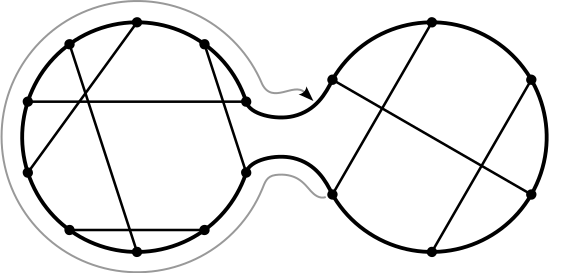
\includegraphics[width=0.27\textwidth, valign=c]{graphics/chord_diagram_connected_sum_result_with_arrow.pdf}
	\]
	Which we show can be achieved by a series of \ref{eq:4T} relations.

	We can rewrite \ref{eq:4T} as
	\[
		\left(
		\ftnorth
		\ - \
		\ftsouth
		\right)
		\ + \
		\left(
		\fteast
		\ - \
		\ftwest
		\right)
		\ = \ 0.
	\]
	A sliding move of our special chosen endpoint of \(a_{2}\) over an endpoint of some chord of \(a_{1}\) is achieved by subtracting the first two terms of the rearranged \ref{eq:4T}. But every chord of \(a_{1}\) is encountered twice in the path. In the other instance it is encountered, the sliding is achieved by subtracting the remaining two terms of \ref{eq:4T}. So, the two connected sums \(a_{1} \connect a_{2}\) differ by a sum of \ref{eq:4T} relations, completing the proof.
     %TODO (ZSuzsi) Given infinite time, a worked example where $a_1$ has one or two chords would be nice
\end{proof}

\begin{proposition}
	The connected sum operation makes \(\mathcal{A}\) into a graded algebra.
\end{proposition}

\begin{proof}
	No chords are lost during the connected sum: the \ref{eq:4T} relation is homogenous with respect to degree, and the connected sum of a chord diagram containing a \ref{eq:1T} chord relation still contains a \ref{eq:1T} chord. So, the connected sum of a chord diagram of order \(i\) and a chord diagram of order \(j\) is a chord diagram of order \(i + j\).
\end{proof}

Just as there is a connected sum operation in \(\mathcal{A}\) reminiscent to that in \(\mathcal{K}\), there is a coproduct too.

\begin{definition}
	\label{def:coproduct-in-chord-diagrams}
	The \textbf{coproduct of a chord diagram} \(A\) is the sum of ways of partitioning its chords between two subdiagrams.  
    Specifically, if \(S\) is the set of chords of \(A\), and \(J \subset S\), let \(\widehat{J} = S \smallsetminus J\). Denote by \(A_{J}\) the chord diagram \(A\) but with only the chords in \(J \subset S\), and the rest deleted. Then
	\[\Delta(A) = \sum_{J \subset S} A_{J} \otimes A_{\overline{J}}.\] %Zsuzsi: I united the two paragraphs here because the second helps the reader not get stuck on the first. (Separate if you don't like)
\end{definition}

\begin{proposition}
	The coproduct \(\Delta\) is well-defined in \(\mathcal{A}\), and makes \(\mathcal{A}\) into a graded bialgebra.
\end{proposition}

\begin{proof}
	We need to check: that the coproduct factors through the quoitents, that the coproduct respects the grading, and that the compatibility condition holds.  %TODO (ZSuzsi) That the coproduct is an algebra morphism (a precise way to say compatibility)

	That \(\Delta\) factors through \ref{eq:1T} is easy: an isolated chord in \(A\) remains isolated and appears in one cofactor of every term of \(\Delta(A)\).
	% TODO: Swap the notation so the 4Ts and 1Ts with stars are in the first chapter and not in the rest.

	Also, \(\Delta\) factors through \ref{eq:4T}. Suppose that \(K = A_{1} - A_{2} + A_{3} - A_{4}\) is some combination of chord diagrams to be killed by \ref{eq:4T}. This means that \(K\) looks like
	\[
		K =
		\left(
		\ftnorth
		\ - \
		\ftsouth
		\right)
		\ + \
		\left(
		\fteast
		\ - \
		\ftwest
		\right)
	\]
	where there may be other chords \(O\) that the above diagrams have in common, as well as those shown. Note that there is one moving chord in the above diagram and one stationary chord. Let us label these \(m\) and \(s\). Take the same partition \(J \sqcup \overline{J}\) of \(S\) for all of the four chord diagrams at once, and write as the resulting coproduct \(\Delta(A_{i}) = C_{i} \otimes D_{i}\). Suppose without loss of generality that \(m\) was partitioned into the \(C_{i}\)'s. Then \(D_{1} = D_{2} = D_{3} = D_{4}\), so this term of the coproduct factors as \((C_{1} - C_{2} + C_{3} - C_{4}) \otimes D_{1}\) and either:
	\begin{itemize}
		\item \(s\) was also partitioned into the \(C_{i}\)'s, and the relation remains a \ref{eq:4T}, or
		\item \(s\) was partitioned into the \(D_{i}\)'s, and so \(C_{1} = C_{2}\) and \(C_{3} = C_{4}\),
	\end{itemize}
	and in either case, that term of the coproduct is killed.

	The coproduct clearly satisfies
	\[\Delta(\mathcal{A}_{m}) \subset \bigoplus_{i + j = m} \mathcal{A}_{i} \otimes \mathcal{A}_{j} = (\mathcal{A} \otimes \mathcal{A})_{m},\]
	so it is graded.

	The compatibility condition holds. If \(A\) has chord set \(S\) and \(B\) has chord set \(T\), then
	\begin{align*}
		\Delta(A) \connect^{\otimes 2} \Delta(B)
		& = \left(\sum_{J' \subset S} A_{J'} \otimes A_{\overline{J'}} \right) \connect^{\otimes 2} \left(\sum_{J'' \subset T} B_{J''} \otimes B_{\overline{J''}} \right) \\
		& = \sum_{J \subset S \sqcup T} (A \connect B)_{J} \otimes (A \connect B)_{\overline{J}} \\
		& = \Delta(A \connect B).
	\end{align*}
\end{proof}

We have shown that \(\mathcal{A}\) is a graded bialgebra of finite type. In fact \(\mathcal{A}\) is an even more specific structure.

\begin{definition}
	A \textbf{connected, commutative, cocommutative} graded bialgebra of finite type is a graded bialgebra, \(A\), of finite type for which
	\begin{itemize}
		\item The unit \(k \to A_{0}\) is an isomorphism (\textbf{connectedness})
		\item The product is commutative, \(m \circ \tau = m\)
		\item The coproduct is cocommutative, \(\tau \circ \Delta = \Delta\)
	\end{itemize}
	% TODO: Define the swap map or check it has been defined before this.
\end{definition}

\begin{proposition}
	The bialgebra \(\mathcal{A}\) is a connected, commutative, cocommutative graded bialgebra of finite type.
\end{proposition}

\begin{shaded}
	\begin{proof}
		The connetedness isomorphism is given by ...

		We have already shown it is commutative.

		The coproduct is clearly cocommutative.
	\end{proof}
\end{shaded}

Connected, commutative, cocommutative graded bialgebras of finite type are very rigid structures. In-particular, a classical strucutral theorem applies, and such a bialgebra can be understood in terms of its primitive elements.

\begin{definition}
	An element \(x\) is \textbf{primitive} in a coalgebra (so in-particular in a bialgebra) with coproduct \(\Delta\) if it satisfies
	\[\Delta(x) = 1 \otimes x + x \otimes 1.\]
	The set of primitive elements of a bialgebra \(A\) is denoted \(\mathcal{P}(A)\), and if \(A\) is graded, then let \(\mathcal{P}_{n}(A)\) denote the set of primitive elements of degree \(n\).
\end{definition}

\begin{theorem}[Milnor-Moore]
	Let \(H\) be a connected, commutative, cocommutative bialgebra of finite type, over a field of characteristic zero. Then, as an algebra, \(H\) is isomorphic to the symmetric algebra of \(\mathcal{P}(H)\). In other words, \(H\) is a polynomial algebra in \(\mathcal{P}(H)\).
\end{theorem}

We refer to \cite{invariants-of-links-and-3-manifolds-from-graph-configurations} or \cite{introduction-to-vassiliev-invariants} for a proof. This fact leads to important consequences about the structure of \(\mathcal{A}\) and its relation to Lie algebras, which will the subject of Chapter \ref{ch:lie-theory-and-jacobi-diagrams}.

\begin{definition}
	The weight systems (Definition \ref{def:weight-system}), denoted \(\mathcal{W}\), form a graded bialgebra, the \textbf{graded bialgebra of weight systems} with grading given by degree \(m\), product given by pointwise multiplication
	\[W_{1}\cdot W_{2}(a) = W_{1}(a)W_{2}(a),\]
	and coproduct, \(\eta\) given by
	\[\eta(W)(a_{1} \otimes a_{2}) = W(a_{1} \connect a_{2}).\]

\end{definition}

In fact, every graded object is a filtered object with the naturally induced filtration. Considering a graded object as such allows us to take its dual filtered bialgebra (which we refer to as its dual graded bialgebra in this case).

\begin{proposition}
	The graded bialgebra \(\mathcal{W}\) is the dual graded bialgebra of the graded bialgebra \(\mathcal{A}\).
\end{proposition}

\section{The fundamental theorem of Vassiliev invariants}
\label{sec:the-fundamental-theorem-of-vassiliev-invariants}

In Section \ref{sec:the-stratification-on-the-space-of-knots-and-integration}, we gave the fundamental theorem of Vassiliev invariants. The point of this theorem is that is establishes a particular relationship between the algebras of the previous two chapters, \(\mathcal{K}\) and \(\mathcal{A}\) (or equivalently, between \(\mathcal{W}\) and \(\mathcal{V}\)). But admittedly, in the form of Theorem \ref{thm:fundamental-theorem-of-vassiliev-invariants}, it's not a-priori obvious why this is the case. Here we give a restatement of that theorem that makes the relationship explicit.

\begin{definition}
	The \textbf{associated graded} algebra of a filtered algebra \(A\) is the algebra formed by the direct sum of the succesive quotients of the filtered components of \(A\). For an algebra with a descending filtration,
	\[\gr A = \bigoplus_{m = 0}^{\infty} A_{m} / A_{m + 1},\]
	and for an algebra with an ascending filtration,
	\[\gr A = \bigoplus_{m = 0}^{\infty} A_{m} / A_{m - 1},\]
	where \(A_{-1} = \{0\}\).
	% TODO: Make bialgebra? Maybe?
    %TODO (Zsuzsi): Yes, you need to explain 1) the algebra structure on grA, and 2) the coalgebra structure. This is especially important becasuse the direct sum is only true as vector spaces, not as algebras.
\end{definition}

\begin{theorem}[Fundamental theorem]
	\label{thm:fundamental-theorem-restated}
	The algebra of weight systems is isomorphic to the associated graded algebra of the algebra of Vassiliev invariants, \(\mathcal{W} \cong \gr \mathcal{V}\), or on the level of graded components,
	\[\bigoplus_{m = 0}^{\infty} \mathcal{W}_{m} \cong \bigoplus_{m = 0}^{\infty} \mathcal{V}_{m} / \mathcal{V}_{m - 1}.\]

	Equivalently, this can be stated in the dual setting as follows. The algebra of chord diagrams is isomorphic to the associated graded algebra of the algebra of knots, \(\mathcal{A} \cong \gr \mathcal{K}\), or on the level of graded components,
	\[\bigoplus_{m = 0}^{\infty} \mathcal{A}_{m} \cong \bigoplus_{m = 0}^{\infty} \mathcal{K}_{m} / \mathcal{K}_{m + 1}.\]
\end{theorem}

We can break the fundamental theorem up into two parts.

\begin{center}
	\begin{tblr}{|Q[c,m]|p{.36\textwidth}|p{.36\textwidth}|}
		\hline
		\textbf{Vassiliev}
		& Every Vassiliev invariant modulo Vassiliev invariants of higher order gives a Weight system, so a map \[\mathcal{V}_{m} / \mathcal{V}_{m - 1} \to \mathcal{W}_{m}.\] \vspace{-20pt}
		& Every chord diagram gives an element of \(\mathcal{K}_{m}\) modulo \(\mathcal{K}_{m + 1}\), so a map \[\mathcal{A}_{m} \to \mathcal{K}_{m} / \mathcal{K}_{m + 1}.\] \vspace{-20pt} \\ \hline
		\textbf{Kontsevich}
		& Every weight system gives a Vassiliev invariant modulo Vassiliev invariants of higher order, so a map \[\mathcal{W}_{m} \to \mathcal{V}_{m} / \mathcal{V}_{m - 1}\] which is inverse to the above.
		& Every equivalence class of \(\mathcal{K}_{m}\) modulo \(\mathcal{K}_{m + 1}\) gives a chord diagram, so a map \[\mathcal{K}_{m} / \mathcal{K}_{m + 1} \to \mathcal{A}_{m}.\] which is inverse to the above. \\ \hline
	\end{tblr}
\end{center}

The equivalence of this version of the theorem with the version (Theorem \ref{thm:fundamental-theorem-of-vassiliev-invariants})given in Section \ref{sec:the-stratification-on-the-space-of-knots-and-integration} will be proven at the end of this section.

The point of the part of this theorem due to Vassiliev is that the relations in \(\mathcal{A}\) are compatible with the relations of \(\mathcal{K}_{n} / \mathcal{K}_{n + 1}\). Indeed, \(\mathcal{A}\) was constructed in this way, and much of that work was already done in Section \ref{sec:the-stratification-on-the-space-of-knots-and-integration}.
% TODO: Find reference for Vassiliev

\begin{proofof}{Theorem \ref{thm:fundamental-theorem-restated} (Vassiliev)}
	For the map \(a \in \mathcal{A}_{m} \to \mathcal{K}_{m} / \mathcal{K}_{m + 1}\) we take the following. 
    %TODO (Zsuzsi) I would rephrase this sentence, $a$ is not a map. Also, perhaos you should first define the map ton $D_m$, and then descend to $A_m$ (which is what you practically do). 
    Given \(a \in \mathcal{A}_{m}\), take a singular knot \(k^{\bullet} \in \singularknots_{m}\) whose chord diagram is \(a\), then
    %TODO (Zsuzsi) switched from present tense to infinitive
    resolving it to an element of \(k \in \mathcal{K}_{m}\), and projecting that into the quotient \(\mathcal{K}_{m} / \mathcal{K}_{m + 1}\).

	This is well-defined since any other \({k^{\bullet}}'\) also has chord diagram \(a\).
    %TODO (Zsuzsi) Any other \({k^{\bullet}}'\) coming from where?
    Any two \(m\)-singular knots with the same chord diagram differ by some crossing changes, in particular this applies to \(k^{\bullet}\) and \({k^{\bullet}}'\). But if \(k^{\bullet}\) and \({k^{\bullet}}'\) differ by a crossing change, then \(\delta^{m}(k^{\bullet})\) and \(\delta^{m}({k^{\bullet}}')\) differ by an element of \(\mathcal{K}_{m + 1}\), so \([\delta^{m}(k^{\bullet})] = [\delta^{m}({k^{\bullet}}')]\). This argument that any \(k^{\bullet} \in \singularknots_{m}\) can be chosen to represent \([\delta^{m}(k^{\bullet})]\)as long as it has chord diagram \(a\) will be used again below, and we refer to it as the crossing-change argument.

	Recalling that \(\mathcal{A}_{m} = \mathcal{D}_{m} / \ref{eq:1T}, \ref{eq:4T}\), we need to show that the map factors through the quotient. Indeed \ref{eq:1T} is in the kernel: a type \ref{eq:1T} chord diagram is sent to a singular knot with a singular point that is passed through twice in a row when the knot is traversed. The resolution, by the crossing-change argument, can be chosen to be a difference of two knots that are isotopic except around the \ref{eq:1T} double point:
    %TODO (Zsuzsi) Make the 1T double point a different colour?
	
	\begin{align*}
		\delta \left(
		
\includegraphics[width=0.255\textwidth, valign=c]{graphics/one_term_isotopy_singularity.pdf}
		\right)
		\,
		& =
		\,
		\includegraphics[width=0.255\textwidth, valign=c]{graphics/one_term_isotopy_positive.pdf}
		\,
		-
		\,
		\includegraphics[width=0.255\textwidth, valign=c]{graphics/one_term_isotopy_negative.pdf} \\ 
		& = \, 0.
	\end{align*}

	Similarly, \ref{eq:4T} is also in the kernel. A combination of chord diagrams appearing in a \ref{eq:4T} relation is sent to a combination of singular knots which by the crossing-change argument can all be chosen to be identical except near a small region, where
	\[
		\tftsouth \ - \ \tfteast \ - \ \tftnorth \ + \ \tftwest
	\]
	but after resolving around the singular point that they don't have in common this becomes 
    %TODO (Zsuzsi) This should not be a single long sentence with a diagrammatic formula in the middle
	\begin{shaded}
		figure of the 8 terms that cancel out.
	\end{shaded}

	% TODO: We here use the definition of Vassiliev invariants as dual to knots. But in the first chapter we actually defined them differently. Can we fix this? Perhaps postponing the definition suffices.

	% TODO: I was tired when I wrote this... I should check it.
	The isomorphism respects the algebra structure as \(a_{1} \connect a_{2}\) is sent to \([k_{a_{1} \connect a_{2}}] \in \mathcal{K}_{m + n} / \mathcal{K}_{m + n + 1}\) that comes from the resolution of a singular knot \(k^{\bullet}_{a_{1} \connect a_{2}}\) with chord diagram \(a_{1} \connect a_{2}\). But likewise \(a_{1}\) and \(a_{2}\) map to \([k_{a_{1}}]\) and \([k_{a_{2}}]\) which are resolutions of singular knots \(k^{\bullet}_{a_{1}}\) and \(k^{\bullet}_{a_{2}}\). The induced operation from the connect sum \(\mathcal{K}_{m}/\mathcal{K}_{m + 1} \otimes \mathcal{K}_{n}/\mathcal{K}_{n + 1} \to \mathcal{K}_{m + n}/\mathcal{K}_{m + n + 1}\) takes these to \([k_{a_{1}} \connect k_{a_{2}}]\), which comes from the resolution of \(k^{\bullet}_{a_{1}} \connect k^{\bullet}_{a_{2}}\). These singular knots may not a-priori be the same, but they have the same chord diagram, so by the crossing-change argument they can be chosen to be the same. Hence their resolutions are the same.

	% TODO: really...?
	Using similar arguments, from the formula of Willerton's Lemma, the isomorphism can be shown to respect the bialgebra structure.

	The dual version of the statement follows from the regular version, but direct proofs are illustrative and we return to them later. %TODO (Zsuzsi) Do you mean you'll show the direct proof of the dual version later?
\end{proofof}

For now, let's turn to the Vassiliev part of the fundamental theorem, with the following definition. %TODO (Zsuzsi) Didn't you just prove the Vassiliev part? When you say "the following definition", a definition should follow.

The part of Theorem \ref{thm:fundamental-theorem-restated} due to Maxim Kontsevich \cite{vassilievs-knot-invariants} is much more involved. Konsevich constructed an integral invariant which proves the fundamental theorem, as well as containing the information of all Vassiliev invariants at the same time. We will not give a detailed exposition of Kontsevich's invariant here, but they abound in the literature, for example \cite{the-fundamental-theorem-of-vassiliev-invariants, the-kontsevich-integral, introduction-to-vassiliev-invariants} in order of increasing level of detail. Rather we will boil the Kontsevich integral down to a single universal property.

\begin{definition}
	The \textbf{completion} of a filtered algebra \(A\) is the filtered algebra
	\[\widehat{A} = \varprojlim_{m \to \infty} A_{m} / A_{m + 1}.\]
    %TODO (Zsuzsi) This sdhould ne $A/A_{m+1}$ (otherwise the inverse limit is not defined)
	In other words this is the degree-completion of the graded algebra \(\gr A\). 
    %TODO (Zsuzsi) This is not true! see notes in email 9th of December
    Note that \(\widehat{A}\) is only a filtered algebra, not a graded one, as its elements can have infinitely many terms non-zero, so it doesn't decompose as a direct sum.
\end{definition}

\begin{definition}
	A \textbf{universal Vassiliev invariant} is a knot invariant \(Z : \mathcal{K} \to \widehat{\mathcal{A}}\) with the following property. If \(k \in \mathcal{K}_{m}\) is a linear combination of knots with \(k = \delta^{m}(k^{\bullet})\) and \(k^{\bullet}\) has chord diagram \(a \in \mathcal{A}_{m}\), then
	\[Z(k) = a + \text{higher degree terms.}\]
\end{definition}

\begin{remark}
	Another equivalent way of defining a universal Vassiliev invariant is as follows. If \(f\) is a descending-filtration-respecting map \(f: A \to B\), then define the associated graded map \(\gr f: \gr A \to \gr B\) that sends \(a_{m} + A_{m + 1} \mapsto f(a_{m}) + B_{m + 1}\). In other words, a graded map coming from the filtered map \(f\) that forgets information about higher degrees. A universal Vassiliev invariant is a map \(Z: \mathcal{K} \to X\) whose associated graded \(\gr Z: \gr \mathcal{K} \to \gr X\) is an isomorphism.

	The Kontsevich integral is such a map with \(X = \widehat{\mathcal{A}}\). In particular, note that \(\gr \widehat{\mathcal{A}} = \mathcal{A}\) (because the direct sum implicit in \(\gr\) means \(a \in \gr \widehat{\mathcal{A}}\) cannot have infinitely many non-zero terms). So since \(Z\) is \(\mathcal{K} \to \widehat{\mathcal{A}}\) and satisfies this property, then \(\gr \mathcal{K} \cong \mathcal{A}\).
\end{remark}

\begin{theorem}[Kontsevich Integral]
	\label{thm:kontsevich-integral-is-universal}
	There exists a universal Vassiliev invariant, denoted \(Z(k)\), called the Kontsevich integral.
\end{theorem}

\begin{proofof}{Theorem \ref{thm:fundamental-theorem-restated} (Kontsevich)}
	Take the map \(k \in \mathcal{K}_{m} \to \mathcal{A}_{m}\) coming from killing the higher degree terms in the Kontsevich integral, and taking the lowest order non-zero chord diagram. This factors through the quotient to a map \(\mathcal{K}_{m}/\mathcal{K}_{m + 1} \to \mathcal{A}_{m}\) since by Theorem \ref{thm:kontsevich-integral-is-universal}, any additional \(k' \in \mathcal{K}_{m + 1}\) contributes only higher degree terms, which get killed. It is easy to see that the two maps are inverses.
\end{proofof}

Again, it's worth looking at the proof in the dual setting too.

\begin{lemma}
	\label{lem:kontsevich-integral-then-weight-system-is-vassiliev}
	Post-composing the Kontsevich integral with a weight system of order \(m\),
	\[k \longmapsto W(Z(k))\]
	(or more precisely, the following composition)
	\[\mathcal{K} \overset{Z}{\longrightarrow} \widehat{\mathcal{A}} \overset{\pi_{m}}{\longrightarrow} \mathcal{A}_{m} \overset{W}{\longrightarrow} \mathbb{Q}\]
	gives a Vassiliev invariant of order \(m\).
\end{lemma}

\begin{proof}
	The map \(W \circ Z\) is clearly an invariant, since \(Z\) is an invariant. It's Vassiliev since on linear combinations \(k \in \mathcal{K}_{m + 1}\), \(Z(k)\) has nothing in degree \(m\), so composing with a weight system of degree \(m\) gives zero.
\end{proof}

\begin{proofof}{Theorem \ref{thm:fundamental-theorem-restated} (dual)}
	The map defined by Lemma \ref{lem:kontsevich-integral-then-weight-system-is-vassiliev},  \(\mathcal{W}_{m} \to \mathcal{V}_{m}\) is injective, as only the zero weight system gives the zero invariant.

	However, it is not surjective. We show that the map, written as
	\[\mathcal{W}_{m} \overset{Z^{\ast}}{\longrightarrow} \mathcal{V}_{m} / \mathcal{V}_{m - 1} \oplus \mathcal{V}_{m - 1}\]
	forces a choice of Vassiliev invariant of degree \(m - 1\). Being as explicit as possible, let
	\[\Omega(k) =
		\begin{cases}
			k \in \mathcal{K}_{m}
			& (W \circ Z)(k)
			\\
			k \notin \mathcal{K}_{m}
			& 0
			\\
		\end{cases},
		\quad \text{and} \quad
	\Theta(k) =
		\begin{cases}
			k \in \mathcal{K}_{m}
			& 0
			\\
			k \notin \mathcal{K}_{m}
			& (W \circ Z)(k)
			\\
		\end{cases},
	\]
	then \(W \circ Z = \Omega + \Theta\), where \(\Omega\) recovers the weight system \(W\), when \(k \in \mathcal{K}_{m}\), and \(\Theta\) is some finite type invariant of order \(m - 1\), determined by \(W\).

	In essence, we have found that the cokernel of \(Z^{\ast}\) is \(\mathcal{V}_{m - 1}\), so we get the desired isomorphism \(\mathcal{W}_{m} \cong \mathcal{V}_{m} / \mathcal{V}_{m - 1}\), at least on the level of vector spaces.
	\end{proofof}

	The natural question arises, what was this summand \(\Theta\)? Fixing \(n < m\) and a knot \(k \in \mathcal{K}_{n}\) with chord diagram \(a_{k}\), it has Kontsevich integral
	\[Z(k) = a_{k} + \parbox{2.5cm}{\centering terms of \\ order \((n + 1)\)} + \cdots + \parbox{1.8cm}{\centering terms of \\ order \(m\)} + \cdots.\]
	Applying the projection \(\pi_{m}\), all that remains are some chord diagrams of order \(m\), with some coefficients depending on the intricacies of the Kontsevich integral for that particular knot. Composing with the weight system, this is a \(\mathbb{Q}\)-valued Vassiliev invariant of order \(m - 1\) determined by \(W\).


The name `universal Vassiliev invariant' we gave to the Kontsevich integrals and invariants of its kind is indeed justified. Every Vassiliev invariant can be obtained through the Kontsevich integral.

\begin{theorem}
	If \(Z\) is a universal Vassiliev invariant, then every Vassiliev invariant factors through \(Z\).
\end{theorem}

\begin{proof}
	Let \(V \in \mathcal{V}_{m}\). Following the proof above, we can project \(V\) to \(\mathcal{V}_{m} / \mathcal{V}_{m - 1}\) to get a weight system \(W_{m}\). Subtracting \(W_{m} \circ Z\) leaves a Vassiliev invariant of one less degree. In other words, via the isomorphism
	\begin{align*}
		\mathcal{V}_{m}
		& \cong \mathcal{V}_{m}/\mathcal{V}_{m - 1} \oplus \mathcal{V}_{m - 1} / \mathcal{V}_{m - 2} \oplus \cdots \oplus \mathcal{V}_{1} / \mathcal{V}_{0} \oplus \mathcal{V}_{0}\\
		& \cong \mathcal{W}_{m} \oplus \mathcal{W}_{m - 1} \oplus \cdots \oplus \mathcal{W}_{1} \oplus \mathcal{W}_{0},
	\end{align*}
	\(V\) can be written as a sequence of weight systems of degree from \(1\) to \(m\) such that \(V\) factors through the Kontsevich integral
	\[V = \sum_{i = 0}^{m} (W_{m} \circ Z) = \left(\bigoplus_{i = 0}^{m} W_{m}\right) \circ Z.\]
\end{proof}

\begin{corollary}
	A universal Vassiliev invariant (in-particular, the Kontsevich integral \(Z\)) is exactly as strong as the set of Vassiliev invariants.
\end{corollary}

\begin{definition}
	Taking the projection \(\mathcal{V}_{m} \to \mathcal{V}_{m}/\mathcal{V}_{m + 1} \cong \mathcal{W}_{m}\) yields a weight system. The \textbf{canonical Vassiliev invariants} are those Vassiliev invariants whose weight systems \(W\) recover them completely via \(W \circ Z\).
\end{definition}

In other words, not all bases of \(\mathcal{V}_{m}\) are created equal. The canonical Vassiliev invariants are those that are homogenous with respect to the splitting of \(\mathcal{V}_{m}\)
\[\mathcal{V}_{m}/\mathcal{V}_{m - 1} \oplus \mathcal{V}_{m - 1} / \mathcal{V}_{m - 2} \oplus \cdots \oplus \mathcal{V}_{1} / \mathcal{V}_{0} \oplus \mathcal{V}_{0}\]
induced by the Kontsevich integral. Canonical Vassiliev invariants were first defined in \cite{on-the-melvin-morton-rozansky-conjecture} and used to prove the Melvin-Morton-Rozansky conjecture relating the coefficients of Alexander polynomial of a knot to those of the coloured Jones polynomials. This is a good example of how the theory of Vassiliev invariants is useful for probing the structure of knots.

\begin{question}[Bar-Natan--Garoufalidis]
	There are a few known from-the-bottom-up constructions of universal Vassiliev invariants of knots. However they are all equivalent to, or conjecturally equivalent to the Kontsevich integral. Yet the Kontsevich integral is not the only invariant that can satisfy the defining degree property of a universal Vassiliev invariant.

	Is there a reason why the Kontsevich integral, or equivalently, this splitting appears to be canonical?
\end{question}

Finally, we return to the equivalence of the two fundamental theorems.

\begin{proof}[Equivalence of Theorems \ref{thm:fundamental-theorem-of-vassiliev-invariants} and \ref{thm:fundamental-theorem-restated}]
	For the forward direction, suppose Theorem \ref{thm:fundamental-theorem-of-vassiliev-invariants} holds. This states that every invariant \(v^{\bullet}\) of \(m\)-singular knots satisfying \ref{eq:T4Tstar} and \ref{eq:T1Tstar} and further that \(\delta v^{\bullet} = 0\), then \(v^{\bullet}\) integrates to an invariant \(v\) of \(0\)-singular knots.

	First we prove that the Kontsevich part of the fundamental theorem holds. Let \(W\) be a weight system of order \(m\). Then \(W\) defines an invariant \(v_{W}^{\bullet}\) of \(m\)-singular knots by \(v_{W}^{\bullet}(k) = W(\sigma(k))\). The derivative of \(v_{W}^{\bullet}\) is zero. Indeed, 
	\[\delta v_{W}^{\bullet}(k) = W(\sigma(k^{+})) - W(\sigma(k^{-}))\]
	for some knots \(k^{+}\) and \(k^{-}\) that differ by crossing changes, but \(\sigma\) is invariant under crossing changes. Also, since \(W\) is a weight system it satisfies \ref{eq:4Tstar} and \ref{eq:1Tstar}, and so \(W'\) satisfies \ref{eq:T4Tstar} and \ref{eq:T1Tstar}. Therefore the conditions of Theorem \ref{thm:fundamental-theorem-of-vassiliev-invariants} and integrates into a Vassiliev invariant.

	The Vassiliev part of the theorem is independent of the original version and was proven separately in Section \ref{sec:the-stratification-on-the-space-of-knots-and-integration}.

	Now for the reverse direction, suppose Theorem \ref{thm:fundamental-theorem-restated} holds. Take a \(m\)-singular knot invariant \(v^{\bullet}\) satisfying \ref{eq:4Tstar} and \ref{eq:1Tstar}, and that \(\delta v^{\bullet} = 0\). This defines a weight system \(W_{v^{\bullet}}\), which by the Kontsevich part of Theorem \ref{thm:fundamental-theorem-restated} gives an invariant class in \(\mathcal{V}_{m} / \mathcal{V}_{m - 1}\). Explicitly, this invariant is \(W_{v^{\bullet}} \circ Z\). But by definition of the derivative of an \(m\)-singular invariant,
		\[
			\delta^{m} (W_{v^{\bullet}} \circ Z)(k^{\bullet})
			=
			(W_{v^{\bullet}} \circ Z)(\delta^{m} k^{\bullet})
		\]
	which by the definition of a universal Vassiliev invariant is just \(v^{\bullet}\).

	Thus, \(W_{v^{\bullet}} \circ Z\) is the \(m\)th derivative of \(v^{\bullet}\), so \(v^{\bullet}\) integrates into a Vassiliev invariant of order \(m\), completing the proof.
\end{proof}


        \chapter{Lie Theory and Jacobi Diagrams}
\label{ch:lie-theory-and-jacobi-diagrams}

% The following sections are simply a list of topics.

\section{(Rooted) Jacobi Diagrams}

\section{Floating Jacobi Diagrams}

\scaffold{In the next section we construct the suprising isomorphism between these two spaces.}

\section{PBW Theorem}

\scaffold{The Poincare-Birkhoff-Witt theorem for Lie algebras has many forms. One of these is that [...] . A corollary of this theorem \cite{enveloping-algebras} is that there is a `canonical' (though, not natural) isomorphism \(S(\mathfrak{g}) \to \mathcal{U}(\mathfrak{g})\) given by \[\omega(x_{1} \cdots x_{n}) = \frac{1}{n!} \sum_{\sigma \in S_{n}} x_{\sigma(1)} \cdots x_{\sigma(n)}.\] Which simply exhibits that fact that \(\operatorname{gr} A \cong A\) unnaturally.}

\scaffold{Futher, \cite{enveloping-algebras}, the two spaces (though not isomorphic as algebras) are isomorphic as \(\mathfrak{g}\)-modules: \(\mathcal{U}(\mathfrak{g})^{\mathfrak{g}} \cong S(\mathfrak{g})^{\mathfrak{g}}\).}

\scaffold{The following theorem is a diagrammatic version of the above.}

\section{Product, Coproduct and Hopf Algebra Structure}

\subsection{Primitive and Grouplike Elements}

\section{Vassiliev Invariants From Lie Algebras with a Metric}


        \chapter{Chord Diagrams as a Universal Enveloping Algebra}
\label{ch:chord-diagrams-as-a-universal-enveloping-algebra}

% Simply a list of topics to cover

\section{Operands and PROPs}

\section{What kinda monoidal category are we in?}

\section{Lie Algebra Objects}

\section{Metrics and Casimir Lie Algebras}

\section{Enveloping Algebras}

\section{External Enveloping Algebra, Internal Enveloping Algebra (?)}



        \chapter{Welded Knots and Arrow Diagrams}
\label{ch:welded-knots-as-arrow-diagrams}

% Simply a list of topics

Question for myself: How does the integration theory change when welded crossings are involved?

\section{Welded knots and spinning}

\section{Arrow diagrams}


        \chapter{Arrow Diagrams as a Universal Enveloping Algebra}
\label{ch:arrow-diagrams-as-a-universal-enveloping-algebra}


        \chapter{Expansions and associators}

\section{First subsection}

\section{Second section}

\section{Third subsection}


        \chapter{Emergent Knotting}
\label{ch:emergent-knotting}


        \chapter{Emergent Welded Associators}
\label{ch:emergent-welded-associators}


        \appendix
        \titleformat{\chapter}[display]
        {\normalfont\bfseries\LARGE}
        {\chaptertitlename~\thechapter}
        {0pc}
        {{\color{black!30!white}\titlerule[0.7pt]}{\color{white}\titlerule[0.7pt]}{\color{black!30!white}\titlerule[0.7pt]}\vspace{0.8pc}\normalfont\Large}

        % \chapter{appendixname}
        % This is the first appendix.

        \emergencystretch=1em
        \newpage
        \printbibliography[title=References]


\end{document}
